\documentclass[
  man,
  longtable,
  nolmodern,
  notxfonts,
  notimes,
  draftfirst,
  colorlinks=true,linkcolor=blue,citecolor=blue,urlcolor=blue]{apa7}

\usepackage{amsmath}
\usepackage{amssymb}




\RequirePackage{longtable}
\RequirePackage{threeparttablex}

\makeatletter
\renewcommand{\paragraph}{\@startsection{paragraph}{4}{\parindent}%
	{0\baselineskip \@plus 0.2ex \@minus 0.2ex}%
	{-.5em}%
	{\normalfont\normalsize\bfseries\typesectitle}}

\renewcommand{\subparagraph}[1]{\@startsection{subparagraph}{5}{0.5em}%
	{0\baselineskip \@plus 0.2ex \@minus 0.2ex}%
	{-\z@\relax}%
	{\normalfont\normalsize\bfseries\itshape\hspace{\parindent}{#1}\textit{\addperi}}{\relax}}
\makeatother




\usepackage{longtable, booktabs, multirow, multicol, colortbl, hhline, caption, array, float, xpatch}
\setcounter{topnumber}{2}
\setcounter{bottomnumber}{2}
\setcounter{totalnumber}{4}
\renewcommand{\topfraction}{0.85}
\renewcommand{\bottomfraction}{0.85}
\renewcommand{\textfraction}{0.15}
\renewcommand{\floatpagefraction}{0.7}

\usepackage{tcolorbox}
\tcbuselibrary{listings,theorems, breakable, skins}
\usepackage{fontawesome5}

\definecolor{quarto-callout-color}{HTML}{909090}
\definecolor{quarto-callout-note-color}{HTML}{0758E5}
\definecolor{quarto-callout-important-color}{HTML}{CC1914}
\definecolor{quarto-callout-warning-color}{HTML}{EB9113}
\definecolor{quarto-callout-tip-color}{HTML}{00A047}
\definecolor{quarto-callout-caution-color}{HTML}{FC5300}
\definecolor{quarto-callout-color-frame}{HTML}{ACACAC}
\definecolor{quarto-callout-note-color-frame}{HTML}{4582EC}
\definecolor{quarto-callout-important-color-frame}{HTML}{D9534F}
\definecolor{quarto-callout-warning-color-frame}{HTML}{F0AD4E}
\definecolor{quarto-callout-tip-color-frame}{HTML}{02B875}
\definecolor{quarto-callout-caution-color-frame}{HTML}{FD7E14}

%\newlength\Oldarrayrulewidth
%\newlength\Oldtabcolsep


\usepackage{hyperref}




\providecommand{\tightlist}{%
  \setlength{\itemsep}{0pt}\setlength{\parskip}{0pt}}
\usepackage{longtable,booktabs,array}
\usepackage{calc} % for calculating minipage widths
% Correct order of tables after \paragraph or \subparagraph
\usepackage{etoolbox}
\makeatletter
\patchcmd\longtable{\par}{\if@noskipsec\mbox{}\fi\par}{}{}
\makeatother
% Allow footnotes in longtable head/foot
\IfFileExists{footnotehyper.sty}{\usepackage{footnotehyper}}{\usepackage{footnote}}
\makesavenoteenv{longtable}

\usepackage{graphicx}
\makeatletter
\newsavebox\pandoc@box
\newcommand*\pandocbounded[1]{% scales image to fit in text height/width
  \sbox\pandoc@box{#1}%
  \Gscale@div\@tempa{\textheight}{\dimexpr\ht\pandoc@box+\dp\pandoc@box\relax}%
  \Gscale@div\@tempb{\linewidth}{\wd\pandoc@box}%
  \ifdim\@tempb\p@<\@tempa\p@\let\@tempa\@tempb\fi% select the smaller of both
  \ifdim\@tempa\p@<\p@\scalebox{\@tempa}{\usebox\pandoc@box}%
  \else\usebox{\pandoc@box}%
  \fi%
}
% Set default figure placement to htbp
\def\fps@figure{htbp}
\makeatother


% definitions for citeproc citations
\NewDocumentCommand\citeproctext{}{}
\NewDocumentCommand\citeproc{mm}{%
  \begingroup\def\citeproctext{#2}\cite{#1}\endgroup}
\makeatletter
 % allow citations to break across lines
 \let\@cite@ofmt\@firstofone
 % avoid brackets around text for \cite:
 \def\@biblabel#1{}
 \def\@cite#1#2{{#1\if@tempswa , #2\fi}}
\makeatother
\newlength{\cslhangindent}
\setlength{\cslhangindent}{1.5em}
\newlength{\csllabelwidth}
\setlength{\csllabelwidth}{3em}
\newenvironment{CSLReferences}[2] % #1 hanging-indent, #2 entry-spacing
 {\begin{list}{}{%
  \setlength{\itemindent}{0pt}
  \setlength{\leftmargin}{0pt}
  \setlength{\parsep}{0pt}
  % turn on hanging indent if param 1 is 1
  \ifodd #1
   \setlength{\leftmargin}{\cslhangindent}
   \setlength{\itemindent}{-1\cslhangindent}
  \fi
  % set entry spacing
  \setlength{\itemsep}{#2\baselineskip}}}
 {\end{list}}
\usepackage{calc}
\newcommand{\CSLBlock}[1]{\hfill\break\parbox[t]{\linewidth}{\strut\ignorespaces#1\strut}}
\newcommand{\CSLLeftMargin}[1]{\parbox[t]{\csllabelwidth}{\strut#1\strut}}
\newcommand{\CSLRightInline}[1]{\parbox[t]{\linewidth - \csllabelwidth}{\strut#1\strut}}
\newcommand{\CSLIndent}[1]{\hspace{\cslhangindent}#1}





\usepackage{newtx}

\defaultfontfeatures{Scale=MatchLowercase}
\defaultfontfeatures[\rmfamily]{Ligatures=TeX,Scale=1}





\title{Can we use the Late Positive Potential to increase the predictive
validity of a formal emotional memory model? A joint neuro-cognitive
approach.}


\shorttitle{LPP in a Formal Emotional Memory Model}


\usepackage{etoolbox}









\authorsnames[{1},{2},{2}]{Robin Hellerstedt,Jordan Gunn,Deborah Talmi}







\authorsaffiliations{
{University},{University of Cambridge}}




\leftheader{Hellerstedt, Gunn and Talmi}






\authornote{ 

\par{       }
}

\makeatletter
\let\endoldlt\endlongtable
\def\endlongtable{
\hline
\endoldlt
}
\makeatother
\RequirePackage{longtable}
\DeclareDelayedFloatFlavor{longtable}{table}

\urlstyle{same}



\usepackage{soul}
\makeatletter
\@ifpackageloaded{caption}{}{\usepackage{caption}}
\AtBeginDocument{%
\ifdefined\contentsname
  \renewcommand*\contentsname{Table of contents}
\else
  \newcommand\contentsname{Table of contents}
\fi
\ifdefined\listfigurename
  \renewcommand*\listfigurename{List of Figures}
\else
  \newcommand\listfigurename{List of Figures}
\fi
\ifdefined\listtablename
  \renewcommand*\listtablename{List of Tables}
\else
  \newcommand\listtablename{List of Tables}
\fi
\ifdefined\figurename
  \renewcommand*\figurename{Figure}
\else
  \newcommand\figurename{Figure}
\fi
\ifdefined\tablename
  \renewcommand*\tablename{Table}
\else
  \newcommand\tablename{Table}
\fi
}
\@ifpackageloaded{float}{}{\usepackage{float}}
\floatstyle{ruled}
\@ifundefined{c@chapter}{\newfloat{codelisting}{h}{lop}}{\newfloat{codelisting}{h}{lop}[chapter]}
\floatname{codelisting}{Listing}
\newcommand*\listoflistings{\listof{codelisting}{List of Listings}}
\makeatother
\makeatletter
\makeatother
\makeatletter
\@ifpackageloaded{caption}{}{\usepackage{caption}}
\@ifpackageloaded{subcaption}{}{\usepackage{subcaption}}
\makeatother

% From https://tex.stackexchange.com/a/645996/211326
%%% apa7 doesn't want to add appendix section titles in the toc
%%% let's make it do it
\makeatletter
\xpatchcmd{\appendix}
  {\par}
  {\addcontentsline{toc}{section}{\@currentlabelname}\par}
  {}{}
\makeatother

%% Disable longtable counter
%% https://tex.stackexchange.com/a/248395/211326

\usepackage{etoolbox}

\makeatletter
\patchcmd{\LT@caption}
  {\bgroup}
  {\bgroup\global\LTpatch@captiontrue}
  {}{}
\patchcmd{\longtable}
  {\par}
  {\par\global\LTpatch@captionfalse}
  {}{}
\apptocmd{\endlongtable}
  {\ifLTpatch@caption\else\addtocounter{table}{-1}\fi}
  {}{}
\newif\ifLTpatch@caption
\makeatother

\begin{document}

\maketitle


\setcounter{secnumdepth}{-\maxdimen} % remove section numbering

\setlength\LTleft{0pt}


\subsection{Introduction}\label{introduction}

Retrieved-context theory (\citeproc{ref-howard2002distributed}{Howard \&
Kahana, 2002}) describes the state-of-the-art in terms of the rules that
govern the chances that an experience we have now will come to mind
later. It is supported by extensive behavioural
(\citeproc{ref-healey2016four}{Healey \& Kahana, 2016};
\citeproc{ref-lohnas2015expanding}{Lohnas et al., 2015};
\citeproc{ref-sederberg2008context}{Sederberg et al., 2008}) and neural
(\citeproc{ref-folkerts2018human}{Folkerts et al., 2018};
\citeproc{ref-kragel2021distinct}{Kragel et al., 2021};
\citeproc{ref-manning2011oscillatory}{Manning et al., 2011};
\citeproc{ref-polyn2005category}{Polyn et al., 2005}) evidence (for a
recent review, see \citeproc{ref-lohnas2021role}{Lohnas \& Healey,
2021}). According to this theory, items become associated with a
gradually-drifting internal context during encoding. This association
functions bidirectionally: retrieving an item reinstates its associated
context, which can then cue further recall. This process accounts for
the tendency to consecutively recall items that were studied nearby in
time (temporal contiguity effects) and, more broadly, items that shared
similar encoding contexts. Polyn et al.
(\citeproc{ref-polyn2009context}{2009}) extended retrieved-context
theory to nontemporal dimensions of context, including pre-experimental
semantic associations and source features that capture shared encoding
conditions. For example, items presented in the same modality share a
source context that promotes their co-recall.

Within this framework, emotional Context-Maintenance and Retrieval
(\citeproc{ref-talmi2019retrieved}{Talmi et al., 2019}) (eCMR) extends
CMR by introducing an emotional dimension of context and by allowing
emotion to modulate encoding strength. The first mechanism captures
emotional similarity among items; the second captures preferential
attention to emotional stimuli. The basis for emotional similarity is
that people process emotional experiences differently than neutral ones
in terms of appraisal (\citeproc{ref-sander2005systems}{Sander et al.,
2005}), attention (\citeproc{ref-pourtois2013brain}{Pourtois et al.,
2013}), physiology (\citeproc{ref-stephens2010autonomic}{Stephens et
al., 2010}) and feelings. Because emotional items share these processing
characteristics, they are more similar to one another than to neutral
items (\citeproc{ref-riberto2022neural}{Riberto et al., 2022}).
Emotionality is represented as a source context dimension. Emotional
items share a common emotional source context and neutral items share a
distinct neutral source context, so that recalling an item from either
category promotes further recall of items from the same category. This
feature is used not only to describe which items are similar to each
other, but also to model the cognitive repercussions of their unique
features.

It is known that emotional items enjoy preferential processing during
encoding (\citeproc{ref-anderson2005affective}{Anderson, 2005};
\citeproc{ref-mackay2004emotion}{MacKay et al., 2004};
\citeproc{ref-pourtois2013brain}{Pourtois et al., 2013};
\citeproc{ref-schupp2006emotion}{Schupp et al., 2006}). eCMR simulates
this by scaling the learning rate for associations from context to item
features (\(M^{CF}\)) during encoding, so that emotional items form
stronger bindings to their encoding context. The degree of extra
processing is governed by the value of parameter \(\Phi_{\text{emot}}\).
When it equals 1, emotional and neutral items receive the same encoding
strength. When it is greater than 1, emotional items are modelled as
receiving extra processing during encoding. Constraining
\(\Phi_{\text{emot}}\) with an independent neural measure, rather than
treating it as a free parameter, would provide a more principled account
of individual differences in emotional memory and a stronger test of the
theory (\citeproc{ref-turner2016more}{Turner et al., 2016}). An
excellent candidate is the late positive potential (LPP), an
event-related potential (ERP) component that increases in amplitude when
participants process emotionally significant visual stimuli
(\citeproc{ref-cuthbert2000brain}{Cuthbert et al., 2000};
\citeproc{ref-hajcak2010event}{Hajcak et al., 2010};
\citeproc{ref-schupp2000affective}{Schupp et al., 2000},
\citeproc{ref-schupp2006emotion}{2006}). In this project, our aim was to
examine the suitability of the LPP for neuro-cognitive modelling of
memory recall. We pursued this aim in three steps: by establishing
individual-level reliability of the LPP under memory-experiment
conditions, by testing whether LPP variation predicts emotional memory,
and by investigating how best to incorporate the neural measure into the
model.

The LPP is broadly characterised as reflecting affective stimulus
significance (\citeproc{ref-hajcak2020significance}{Hajcak \& Foti,
2020}; \citeproc{ref-olofsson2008affective}{Olofsson et al., 2008}), and
its emotional modulation has been observed at the group level across a
range of stimuli and presentation durations. However, to constrain
individual participants' model parameters, the LPP must also
differentiate emotional from neutral processing at the individual level.
Recently, Schupp and Kirmse (\citeproc{ref-schupp2021case}{2021})
examined individual-level sensitivity to emotional content using a
case-by-case approach across three studies with different emotional
stimulus categories. They observed that the LPP was larger for high-
compared to low-arousing stimuli in 98\% of individual-level tests, and
a complementary specificity analysis confirmed that this effect was
driven by emotional content rather than low-level stimulus differences.
Because eCMR attributes the emotional encoding advantage to preferential
processing during study, and the LPP is sensitive to the enhanced
processing of motivationally significant stimuli, these findings
motivate testing whether LPP variation can usefully constrain
\(\Phi_{\text{emot}}\).

For the LPP to serve this constraining role, however, the same
individual-level reliability must hold under conditions typical of
memory experiments. Although emotional modulation of the LPP has been
observed at the group level in intentional-encoding paradigms followed
by free recall (\citeproc{ref-barnacle2018context}{Barnacle et al.,
2018}), it is not yet known whether comparable individual-level
sensitivity is preserved. Participants in Schupp and Kirmse
(\citeproc{ref-schupp2021case}{2021})'s study encoded briefly-presented
pictures passively. By contrast, participants in typical memory recall
experiments are aware of an upcoming memory test. Intentional encoding
instructions could dilute the emotional modulation of the LPP in several
ways. Participants may shift attention from processing each stimulus in
isolation to comparing stimuli or organising them for later recall. They
may also adopt encoding strategies that reduce processing differences
between emotional and neutral items, or engage in rehearsal that
redistributes attention more evenly across stimulus types. The potential
impact of encoding mode is supported by evidence that task demands
modulate emotional ERP effects
(\citeproc{ref-schindler2020selective}{Schindler \& Straube, 2020}) and
that encoding instructions alter the organisation of recall
(\citeproc{ref-healey2019contiguity}{Healey et al., 2019}). Our first
aim, therefore, was to replicate Schupp and Kirmse
(\citeproc{ref-schupp2021case}{2021})'s findings using a setup more
typical in memory research. In addition to testing whether the LPP's
emotional modulation survives intentional encoding, a replication would
increase confidence in the generality of the findings. Relative to
Schupp and Kirmse (\citeproc{ref-schupp2021case}{2021}), the present
study uses a different stimulus set, a longer presentation duration (2 s
vs.~150 ms), and a larger sample (\emph{n} = 38).

Beyond individual-level reliability, our second aim was to examine
whether the emotional modulation of the LPP predicts the emotional
modulation of memory. Attention and memory are typically coupled, such
that when all else is held equal, increased attention during encoding
increases participants' ability to recall attended stimuli subsequently
(\citeproc{ref-chun2007interactions}{Chun \& Turk-Browne, 2007}).
Increased attention to emotional stimuli during encoding is considered a
key driver of enhanced memory for these stimuli
(\citeproc{ref-mather2011arousal}{Mather \& Sutherland, 2011};
\citeproc{ref-talmi2013enhanced}{Talmi, 2013}). Accordingly, previous
studies report that emotional arousal increased both LPP and memory
(\citeproc{ref-dolcos2002event}{Dolcos \& Cabeza, 2002}). Yet direct
tests of whether the LPP--memory relationship is consistent within or
between subjects are scarce (\citeproc{ref-fields2023p300}{Fields,
2023}). Indeed, Barnacle et al.
(\citeproc{ref-barnacle2018context}{2018}) found that the emotional
modulation of the LPP was equally strong in pure and mixed lists under
intentional encoding conditions, despite the fact that emotional memory
enhancement was context-dependent. These results suggest a functional
dissociation between attention-related LPP modulation and the downstream
memory advantage. Understanding how LPP variation relates to memory
within a mechanistic model may help bridge this gap. At the
between-subjects level, individuals with larger emotion-dependent LPP
differences may exhibit larger emotion-dependent memory differences. At
the within-subject level, individuals may recall best those specific
lists where encoding was accompanied by a larger LPP. The dissociation
between within- and between-subject effects in ERPs was recently
demonstrated for the left parietal old-new effect, where robust
within-subject effects were observed despite null between-subject
effects (\citeproc{ref-macleod2017left}{MacLeod \& Donaldson, 2017}).
Although the emotional modulation of the LPP shows good internal
consistency (\citeproc{ref-moran2013psychometric}{Moran et al., 2013})
and is reliable within individuals across testing sessions
(\citeproc{ref-weinberg2021emotion}{Weinberg et al., 2021}), it is
unknown whether this reliability extends to predicting memory
differences. If trial-level LPP variation tracks encoding-related
processing relevant to \(\Phi_{\text{emot}}\), the model predicts a
positive association between the emotional modulation of the LPP and the
emotional recall advantage, at the within-subject level, the
between-subjects level, or both (Figure 1).

In addition, we wanted to investigate whether the relation between the
LPP and emotion enhanced memory is better captured on the single-trial
level or when averaged over all the items in a list to decide at what
level we should add the LPP to the eCMR. It could for example be that
the LPP is too noisy at the single-trial level to be useful, or that the
loss of variability in LPP amplitude between items after averaging leads
to a weaker relationship between the LPP and emotion enhanced memory. It
was therefore important to examine at what level the relationship
between the LPP and subsequent memory is stronger to inform our
modelling decisions.

Finally, we used these results to constrain a process model of memory
encoding and retrieval. CMR captures temporal-context encoding and
retrieval but has no emotion mechanism, and so provides a floor. CMR+LPP
tests whether the LPP can serve as a substitute for category labels: it
uses the same single-context architecture as CMR but scales encoding
strength by trial-level LPP amplitude without any emotional context
dynamics. eCMR adds an emotional context layer and emotion-modulated
encoding strength, using only category labels. LPP-eCMR translates the
emotion-specific LPP effect identified by the GLMM into the model's
per-item encoding-strength term. The comparison tests whether
trial-level LPP can substitute for category labels, whether embedding
the LPP in a mechanistic retrieval model improves prediction beyond what
category labels alone provide, and whether the resulting model generates
qualitatively distinct predictions about neural-behavioral
relationships. Because the cognitive model is fit to each participant
independently, it can reveal whether the LPP's contribution to
prediction is consistent across individuals or concentrated in a subset.

The four models cross two dimensions: the presence or absence of an
emotional context layer (which uses category labels to distinguish
emotional from neutral items) and the use of trial-level LPP to modulate
encoding strength. CMR+LPP and eCMR share the same parameter count
(\(k = 10\)), differing only in whether emotional memory is driven by a
continuous neural signal or categorical source features. eCMR and
LPP-eCMR share identical architecture, differing only in how LPP enters
the encoding-strength term, so differences in predictive performance
between them are attributable to the LPP term alone. Comparing
alternatives that differ in retrieval dynamics would require
output-order information that the present data lack.

\subsection{Method}\label{method}

This secondary data analysis is based on data from Zarubin et al.
(\citeproc{ref-zarubin2020contributions}{2020}). A more detailed
description of the methods in the original experiment is provided in
paper.

\subsubsection{Participants}\label{participants}

The forty included participants from the mixed condition in Zarubin et
al. (\citeproc{ref-zarubin2020contributions}{2020}) were re-analysed.
One participant was excluded for missing data from three lists and one
participant was excluded due to having fewer than 16 trials in one of
the subsequent memory conditions. The final sample consisted of 38
participants (28 females, \emph{M}\textsubscript{age} = 20,
\emph{SD}\textsubscript{age} = 1.07). Gender and age data was missing
for one of the participants. All participants provided written informed
consent and the experiment was approved by Wofford College Institutional
Review Board (\citeproc{ref-zarubin2020contributions}{Zarubin et al.,
2020}).

\subsubsection{Materials}\label{materials}

There were 22 pictures in each list and nine lists in the whole
experiment. The first two pictures were used as fillers to control for
primacy effects and were excluded from data analysis. The pictures were
selected from the International Affective Picture System
(\citeproc{ref-lang2005international}{Lang et al., 2005}), the Geneva
Affective Picture Database
(\citeproc{ref-danglauser2011geneva}{Dan-Glauser \& Scherer, 2011}), the
Emotional Picture Set (\citeproc{ref-wessa2010emopics}{Wessa et al.,
2010}), the image pool of Talmi et al.
(\citeproc{ref-talmi2007contribution}{2007}) and Google Images. The
pictures were either of negative valence or neutral valence. The neutral
condition was divided into semantically unrelated and semantically
related neutral pictures in the original study, but they were collapsed
in this secondary data analysis to increase the number of trials in the
neutral condition.

\subsubsection{Procedure}\label{procedure}

The participants studied 22 pictures shown consecutively on the screen
for 2000 ms with a 4000 ms inter-trial interval, intended to reduce
emotional carryover effects (\citeproc{ref-talmi2012accounting}{Talmi \&
McGarry, 2012}). The presentation order of both the lists and the images
within lists was randomised. A one minute arithmetic distracter task
followed immediately after the study task to reduce rehearsal of the
pictures and recency effects. A verbal recall test followed the
distracter task. The participants were instructed to recall images only
from the list that they had just seen. The participants had three
minutes to recall the images from the study phase, but could stop sooner
if they had no more items to report.

\subsubsection{EEG pre-processing}\label{eeg-pre-processing}

Raw EEG files were downloaded from the open science framework page for
the Zarubin et al. (\citeproc{ref-zarubin2020contributions}{2020})
study. The EEG was pre-processed with the EEGLAB toolbox in MATLAB
(\citeproc{ref-delorme2004eeglab}{Delorme \& Makeig, 2004}). The data
was re-referenced offline to the average of the left and right mastoid
electrodes and filtered between 0.1 and 40Hz with a band pass FIR
filter. The data was time-locked to the stimulus and segmented into
epochs from −2000 ms to 3000 ms post stimulus onset. The epochs were
baseline corrected using a pre-stimulus time window from −200 ms to 0
ms. Customized threshold functions from the FASTER toolbox
(\citeproc{ref-nolan2010faster}{Nolan et al., 2010}) were used to detect
and reject bad channels and bad epochs based on participant-level
z-transformed values over trials and electrodes that exceeded ± 3.
Independent component analysis was used to correct for EOG artefacts, by
manually removing components classified as blinks, horizontal or
vertical eye-movements. Bad channels which were deleted prior to ICA
were interpolated after the ICA cleaning. In addition, bad channels
within single epochs were detected and interpolated with a criterion of
±3 SD. All participants contributed at least 16 trials in each of the
four ERP conditions. The mean number of trials was 30.7 (\emph{SD} =
6.08) in the negative remembered condition, 26.1 (\emph{SD} = 5.54) in
the negative forgotten condition, 48 (\emph{SD} = 15.33) in the neutral
remembered condition and 66.5 (\emph{SD} = 16.93) in the neutral
forgotten condition after pre-processing. Trials that were rejected
during EEG preprocessing were excluded from the behavioural analyses as
well to ensure that the EEG and behavioural data contained the same
trials and to increase the chance of finding a relation between the two
measures.

\subsubsection{Behavioural Data
Analysis}\label{behavioural-data-analysis}

We investigated whether there was an emotion enhanced memory effect by
comparing the proportion of negative items recalled and the proportion
of neutral items recalled with a paired t-test.

\subsubsection{EEG Data Analysis}\label{eeg-data-analysis}

\paragraph{Focal ERP Analysis.}\label{focal-erp-analysis}

We first analysed the electrodes and time windows where the LPP is
typically maximal in the literature. Averaged EEG amplitude was
extracted from four centroparietal electrodes, Cz, CP1, CP2 and Pz, in
an early time window between 400--1000 ms and a late time window between
1000--2000 ms post stimulus onset. We extracted the EEG amplitudes
separately for subsequently remembered and subsequently forgotten trials
for both the negative and the neutral condition. All mixed effects model
analyses were conducted using the lme4 package in R
(\citeproc{ref-bates2015lme4}{Bates et al., 2015}).

We first performed a linear mixed effects model to analyse if ERP
amplitude was predicted by emotion and subsequent memory. In this model
we used ERP amplitude as the dependent variable, Emotion (Negative vs
Neutral) and Subsequent memory (Remembered vs Forgotten) as fixed
effects, and random intercept + random slope effects of participant. The
formula was:

\[\text{ERP amplitude} \sim 1 + \text{Emotion} \times \text{Memory} + (1 + \text{Emotion} \times \text{Memory} \mid \text{Participant})\]

The random effect structure needed to be simplified to only include a
random intercept effect of participant in the late LPP time window due
to a warning of singular fit. The statistical significance of the fixed
effects and their interaction was assessed using \(\chi^2\) Wald test as
implemented in the car package (\citeproc{ref-fox2019companion}{Fox \&
Weisberg, 2019}). Significant interactions were followed-up using
pairwise contrasts as implemented in the emmeans package in R
(\citeproc{ref-lenth2024emmeans}{Lenth, 2024}) applying a Benjamini \&
Hochberg (false discovery rate, FDR) correction for multiple
comparisons.

\paragraph{Global ERP Analysis.}\label{global-erp-analysis}

We complemented the focal analysis with a global data-driven analysis
including all data points between 0 and 2000 ms, the time window when
the stimulus was presented. The reason for including this analysis is
that analysing ERP data from a small group of electrode sites and time
windows may overlook effects at other electrode sites and time windows.
In this analysis we controlled for multiple comparisons using
cluster-based permutation tests as implemented in the FieldTrip toolbox
(\citeproc{ref-maris2007nonparametric}{Maris \& Oostenveld, 2007};
\citeproc{ref-oostenveld2011fieldtrip}{Oostenveld et al., 2011}). The
first step of this analysis is to perform \emph{t}-tests at every ERP
data sample. Significant samples, uncorrected at \(\alpha\) = .05, that
were neighbours in time or space, including at least two electrodes,
were grouped into clusters. The cluster level t-value was computed by
calculating the sum of the t-values from all samples included in the
cluster. Finally, we compared the cluster level \emph{t}-value in the
observed data to the size of the maximal cluster in 5000 permutations,
for which the datapoints were randomly swapped between conditions within
participants. The cluster level Monte-Carlo \emph{p}-value was
calculated as the proportion of the permutations for which the maximum
cluster was larger than the clusters in the observed data. The exact
spatio-temporal distribution of the clusters should be interpreted with
caution given that the correction for multiple comparisons are applied
at the cluster level rather than at the individual sample level
(\citeproc{ref-sassenhagen2019cluster}{Sassenhagen \& Draschkow, 2019}).

\paragraph{Bootstrap Analysis.}\label{bootstrap-analysis}

To be useful for the purpose of model constraint, the LPP needs to be
reliable within subjects. We therefore performed a bootstrap analysis to
assess the reliability of the Negative--Neutral difference within each
participant's data. The rationale of this analysis is that negative
stimuli should elicit a more positive LPP than neutral stimuli
independent of which specific trials contributed to calculating the
ERPs.

The number of trials was first equated for the two conditions with
undersampling. The data included in this analysis was extracted from the
same centro-parietal electrode sites as in the focal ERP analysis, i.e.
Cz, CP1, CP2 and Pz. Bootstrap resampling from single trials was used to
create a distribution of 1000 resampled ERPs per condition. A sliding
time window was applied to detect the most positive LPP peak (the mean
amplitude of the 100 ms time window between 400--1000 ms for the early
LPP and between 1000--2000 ms for the late LPP). Difference scores were
calculated by subtracting the amplitude in the neutral condition from
the amplitude in the negative condition for each bootstrap sample. Next,
the proportion of positive bootstrap differences were calculated for the
two time-windows based on the rationale that participants with robust
LPP effects should have a large proportion of positive bootstrapped
differences.

We interpreted the emotion enhanced LPP as being reliable if a
proportion of 0.9 or more of the bootstrapped differences were positive
because this cutoff has been used in similar analyses in the concealed
information test literature (for example
\citeproc{ref-rosenfeld2019p300}{Rosenfeld, 2020}).

\paragraph{Relationship between the LPP and Emotion Enhanced
Memory.}\label{relationship-between-the-lpp-and-emotion-enhanced-memory}

The ERPs were z-transformed using the mean and the standard deviation of
a pre-stimulus interval from −200 to 0 ms. This was done on a
single-trial level and separately for all electrodes. Next, the
z-transformed LPP was extracted from the same centroparietal electrodes
as in the focal ERP analysis for both the early, 400--1000 ms, and the
late, 1000--2000 ms, time window.

In the between subjects correlation, we calculated the average LPP and
memory performance across the 9 lists and computed a negative--neutral
difference score in both measures. These measures were then correlated
using Bayesian Pearson correlation.

Besides this between subject correlation we also calculated a
within-subject correlation. In this analysis, we correlated the emotion
enhanced LPP with the emotion enhanced memory across the 9 lists and
calculated the average correlation coefficient across lists for each
participant with Pearson correlation. Next, we performed a Bayesian
one-sample \emph{t}-test against zero to test if there was a
correlation.

Finally, we investigated the relation between memory performance and the
LPP on the single-trial level with a binomial generalized linear
mixed-effect model where we investigated if Subsequent memory was
predicted by Emotion and LPP amplitude. In this model we used Subsequent
memory as the dependent variable and included Emotion (Negative vs
Neutral) and LPP amplitude as fixed effects and random intercept +
random slope effects of Participant. The model formula was:

\[\text{Memory} \sim 1 + \text{Emotion} \times \text{LPP} + (1 + \text{Emotion} \times \text{LPP} \mid \text{Participant})\]

\subsection{eCMR Specification}\label{ecmr-specification}

Building on the behavioural and ERP results reported above, we test
mechanistic accounts of how the LPP can modulate encoding within the
eCMR framework (\citeproc{ref-talmi2019retrieved}{Talmi et al., 2019}).
We embed the Early LPP as an item-level modulator of emotional encoding
strength and compare three variants that differ only in how LPP enters
this term.

We use the full eCMR architecture, which maintains two parallel context
layers --- a temporal context \(c^{T}\) and an emotional context
\(c^{E}\) --- with separate bidirectional association matrices for each
pathway. Items are represented by one-hot feature vectors \(f_{i}\).
Each item also carries a binary source feature \(s_{i}\) that codes
emotional category: \(s_{i} = [1, 0]\) for emotional items and
\(s_{i} = [0, 1]\) for neutral items. All model variants share this
dual-context architecture; they differ only in how LPP modulates
encoding strength within the emotional pathway.

The temporal pathway includes feature-to-context associations \(M^{FC}\)
(items to temporal context) and context-to-feature associations
\(M^{CF}\) (temporal context to items). The emotional pathway includes
analogous associations \(M^{FC}_{emot}\) (items to emotional context)
and \(M^{CF}_{emot}\) (emotional context to items).

\begin{table}

{\caption{{Parameters and structures specifying
eCMR.}{\label{tbl-params}}}
\vspace{-20pt}}

\begin{longtable}[]{@{}
  >{\raggedright\arraybackslash}p{(\linewidth - 2\tabcolsep) * \real{0.4306}}
  >{\raggedright\arraybackslash}p{(\linewidth - 2\tabcolsep) * \real{0.5694}}@{}}
\toprule\noalign{}
\begin{minipage}[b]{\linewidth}\raggedright
Symbol
\end{minipage} & \begin{minipage}[b]{\linewidth}\raggedright
Meaning
\end{minipage} \\
\midrule\noalign{}
\endhead
\bottomrule\noalign{}
\endlastfoot
\(c^{T}\) & temporal context \\
\(c^{E}\) & emotional context \\
\(f_{i}\) & item feature vector (one-hot) \\
\(s_{i}\) & source feature vector (2-unit localist) \\
\(M^{FC}\), \(M^{CF}\) & temporal pathway associations \\
\(M^{FC}_{emot}\), \(M^{CF}_{emot}\) & emotional pathway associations \\
\(\beta_{enc}\) & temporal encoding drift rate \\
\(\beta_{emot}\) & emotional encoding drift rate \\
\(\beta_{start}\) & start-list drift rate \\
\(\beta_{rec}\) & recall drift rate \\
\(\alpha\) & shared support in \(M^{CF}\) \\
\(\delta\) & self-support in \(M^{CF}\) \\
\(\gamma\) & learning rate for \(\Delta M^{FC}\) \\
\(\phi_{s}\) & primacy scale \\
\(\phi_{d}\) & primacy decay \\
\(\tau_{c}\) & choice sensitivity \\
\(\phi_{emot,i}\) & emotional encoding strength \\
\(L_{i}\) & list-centered Early LPP \\
\(\kappa_{L}, \lambda_{L}\) & LPP main-effect slope, offset \\
\(\kappa_{EL}, \lambda_{EL}\) & LPP-by-emotion slope, offset \\
\end{longtable}

\end{table}

Pre-experimental memory is initialized as

\[M_{pre(ij)}^{FC} = \left\{ \begin{matrix}
1 - \gamma & \text{if }i = j \\
0 & \text{if }i \neq j
\end{matrix} \right.\ \]

\[M_{pre(ij)}^{CF} = \left\{ \begin{matrix}
\delta & \text{if }i = j \\
\alpha & \text{if }i \neq j
\end{matrix} \right.\ \]

Emotional associations link each item to its category's context pole:
emotional items associate with the emotional pole and neutral items with
the neutral pole. Pre-experimental weights are \((1 - \gamma)\) for
\(M^{FC}_{emot}\). \(M^{CF}_{emot}\) is initialized to zero; all
emotional context-to-item associations develop through encoding.

During encoding, temporal contextual input is retrieved as
\(c_{i}^{IN} = M^{FC}f_{i}\) and normalized to unit length. Temporal
context updates according to

\[c_{i}^{T} = \rho_{i}c_{i - 1}^{T} + \beta_{enc}c_{i}^{IN}\]

\[\rho_{i} = \sqrt{1 + \beta_{enc}^{2}\left\lbrack \left( c_{i - 1}^{T} \cdot c_{i}^{IN} \right)^{2} - 1 \right\rbrack} - \beta_{enc}\left( c_{i - 1}^{T} \cdot c_{i}^{IN} \right)\]

Emotional context drifts toward the presented item's category pole via
\(c_{i}^{E,IN} = M^{FC}_{emot}f_{i}\):

\[c_{i}^{E} = \rho_{i}^{E}c_{i - 1}^{E} + \beta_{emot}c_{i}^{E,IN}\]

with \(\rho_{i}^{E}\) computed analogously. Both emotional and neutral
items update emotional context, pushing it toward the emotional or
neutral pole respectively.

Feature-to-context learning proceeds identically for both pathways:

\[\Delta M^{FC} = \gamma f_{i}c^{T\top}_{i}, \quad \Delta M^{FC}_{emot} = \gamma f_{i}c^{E\top}_{i}\]

The primacy-graded attention term is:

\[\phi_{i} = \phi_{s}e^{- \phi_{d}(i - 1)} + 1\]

Following Talmi et al. (\citeproc{ref-talmi2019retrieved}{2019}, Eq.
11), context-to-feature learning differs between pathways. The temporal
pathway uses primacy only:

\[\Delta M^{CF} = \phi_{i} \cdot c^{T}_{i}f_{i}^{\top}\]

The emotional pathway is additionally scaled by the per-item emotional
encoding strength \(\phi_{emot,i}\):

\[\Delta M^{CF}_{emot} = \phi_{i} \cdot \phi_{emot,i} \cdot c^{E}_{i}f_{i}^{\top}\]

The parameterization of \(\phi_{emot,i}\) defines each model variant
(see below). Negative values of \(\phi_{emot,i}\) are clamped to 0.

At recall onset, both contexts are shifted toward their respective
pre-list states with drift rate \(\beta_{start}\). At each recall step,
temporal and emotional contexts jointly cue item activations:

\[A_{i} = \left(M^{CF}c^{T}\right)_{i} + \left(M^{CF}_{emot}c^{E}\right)_{i}\]

\[P(i) = \frac{A_{i}^{\tau_{c}}}{\sum_{k}^{}A_{k}^{\tau_{c}}}\]

After recall, the retrieved item's context is reinstated in both
pathways via \(M^{FC}\) and \(M^{FC}_{emot}\), each integrated with
drift rate \(\beta_{rec}\). To simplify model evaluation, we omit an
explicit termination mechanism; instead, we match each trial's observed
output length during simulation. Model evaluation thus focuses on
predicting the composition of recall sets across trials.

\subsubsection{Model Variants}\label{model-variants}

We compare four models that cross two factors: the emotional context
architecture (absent vs.~present) and the information source for
encoding modulation (LPP vs.~category labels). Let \(e_{i}\) be an
indicator that equals 1 for emotional items and 0 for neutral items, and
let \(L_{i}\) denote the trial-mean-centered Early LPP amplitude for
item \(i\).

The base model, CMR (\(k = 9\)), includes temporal context only. No
emotional context layer is included and no emotion parameters are
estimated.

CMR+LPP (\(k = 10\)) uses the same single-context architecture as CMR
but adds one parameter \(\kappa_{L}\) scaling trial-level Early LPP
amplitude into encoding strength:

\[\phi_{emot,i} = \kappa_{L} \cdot L_{i}\]

The encoding modulation applies to all items regardless of category and
operates through the temporal context-to-feature pathway \(M^{CF}\).
This model tests whether a continuous neural measure of encoding-related
processing, without any category labels or emotional context dynamics,
can account for emotional memory effects.

eCMR (\(k = 10\)) takes a different approach: rather than continuous
neural measures, it adds the emotional context layer described above
with one additional parameter \(\phi_{emot}\) controlling
emotion-modulated encoding strength:

\[\phi_{emot,i} = \phi_{emot} \cdot e_{i}\]

The model distinguishes emotional from neutral items via category labels
but has no access to trial-level neural measures.

LPP-eCMR (\(k = 11\)) adds one parameter \(\kappa_{EL}\) scaling the
Early LPP's contribution to emotional encoding strength:

\[\phi_{emot,i} = \phi_{emot} \cdot e_{i} + \kappa_{EL} \cdot L_{i} \cdot e_{i}\]

The \(e_{i}\) term restricts the LPP's influence to emotional items,
directly mapping the GLMM finding (\(\beta\) = .14, \emph{p} \textless{}
.001 for emotional; \(\beta\) = .01, \emph{p} = .488 for neutral). A
main-effect LPP term is omitted because the GLMM found no LPP--recall
association for neutral items, and trial-mean-centering of \(L_{i}\)
absorbs any threshold offset.

The four models form two nested pairs: CMR nests under CMR+LPP (setting
\(\kappa_{L} = 0\)), and eCMR nests under LPP-eCMR (setting
\(\kappa_{EL} = 0\)). CMR+LPP and eCMR are not nested because they
differ in architecture (single vs.~dual context) and information source
(LPP vs.~category labels). At \(k = 10\), the comparison between CMR+LPP
and eCMR tests whether trial-level LPP can replace category labels at
equal parameter cost.

\subsubsection{Evaluation Approach}\label{evaluation-approach}

We evaluated each model by how well it predicts the unordered set of
recalled items on each list (not recall order), because our data is
missing recall order information and because our primary behavioral
outcomes and benchmarks target item selection rather than
order-dependent dynamics. Let \(S_{t}\) denote the set of items recalled
on trial \(t\), and let \(r\) range over recall sequences that contain
exactly the items in \(S_{t}\) (in any order). We define the \emph{set
likelihood} as

\[P\left( S_{t} \mid \theta \right) = \sum_{r:\, r\ \text{yields}\ S_{t}}^{}P(r \mid \theta),\]

where \(\theta\) are the model parameters.

Evaluating this sum exactly is infeasible because the number of
sequences that yield a given set grows rapidly with
\(\left| S_{t} \right|\). We therefore approximate
\(P\left( S_{t} \mid \theta \right)\) by Monte Carlo sampling: for each
trial we draw \(K\) random permutations \(r_{1},\ldots,r_{K}\) of
\(S_{t}\), compute \(P\left( r_{k} \mid \theta \right)\), and estimate
the sum as
\(\left| S_{t} \right|!\,\frac{1}{K}\sum_{k = 1}^{K}P\left( r_{k} \mid \theta \right)\).
Because the factorial factor does not depend on \(\theta\), we maximize
the (unscaled) mean permutation likelihood
\(\frac{1}{K}\sum_{k}^{}P\left( r_{k} \mid \theta \right)\), which is
proportional to the set likelihood and yields identical fits and
\(\Delta\)AIC comparisons.

We maximize the objective with differential evolution
(\citeproc{ref-storn1997differential}{Storn \& Price, 1997}). Because
the optimizer is stochastic, we run three independent fits per
participant and model variant and retain the best-performing fit. We
compare models using AIC computed from the approximate set
log-likelihood. For nested model pairs, we floor the child model's
per-subject NLL at the parent model's value to correct for occasional
optimizer failures that would otherwise violate the nesting guarantee.
In addition to AIC weights and pairwise \(\Delta\)AIC, we report
Bayesian model selection {[}BMS; Stephan et al.
(\citeproc{ref-stephan2009bayesian}{2009}){]} with protected exceedance
probabilities (\citeproc{ref-rigoux2014bayesian}{Rigoux et al., 2014})
to characterize population-level model frequencies. We judge a pairwise
\(\Delta\)AIC advantage as reliable when its 95\% CI excludes zero. For
BMS, an exceedance probability above .95 provides strong evidence that
one model is the most frequent in the population; values near chance
(\(1/M\) for \(M\) models) indicate that the data do not distinguish
models at the population level. We then assess qualitative adequacy by
simulating each fitted model on the study lists while matching each
trial's observed output length and plotting the benchmark summaries.
This set-likelihood approach evaluates models on their ability to
reproduce the full recalled sets, providing a stringent test of
mechanistic hypotheses.

\subsection{Results}\label{results}

\subsubsection{Behavioural Results}\label{behavioural-results}

Replicating the original analysis, a paired t-test showed that memory
performance was significantly higher for negative items (\emph{M} =
0.54, \emph{SD} = 0.1) compared to neutral items (\emph{M} = 0.42,
\emph{SD} = .14), \emph{t}(37) = 6.18, \emph{p} \textless{} .001.

\hl{For the record. If we run a one-way repeated measures ANOVA with
proportion remembered as the dependent variable and condition (Negative
vs Category vs Neutral) as the independent variable, we get a
significant effect \emph{F}(1,65) = 42.85, \emph{p} \textless{} .001,
partial eta squared = 0.54. Follow up pairwise comparisons shows that
Negative items were remembered more than both category items
(\emph{t}(37) = 2.46, \emph{p} = .01) and neutral items (\emph{t}(37) =
9.41, \emph{p} \textless{} .001). Memory performance was also higher for
category items (semantically related neutral items) than for neutral
items (semantically unrelated neutral items; (\emph{t}(37) = 7.29,
\emph{p} \textless{} .001). The pattern of results was hence Negative
\textgreater{} Category \textgreater{} Neutral.}

\subsubsection{EEG Results}\label{eeg-results}

\paragraph{Focal ERP Analysis.}\label{focal-erp-analysis-1}

A linear mixed effect model was conducted to investigate if Emotion
(Negative vs Neutral) and Subsequent memory (Remembered vs Forgotten)
predicted ERP amplitude was conducted separately for the early and the
late LPP time window.

In the early time window, there was a main effect of Emotion (\(\beta\)
= .10, \(\chi^2\)(1) = 6.84, \emph{p} = .009) and a main effect of
Subsequent memory (\(\beta\) = .25, \(\chi^2\)(1) = 26.70, \emph{p}
\textless{} .001) and a significant Emotion x Subsequent memory
interaction (\(\beta\) = .20, \(\chi^2\)(1) = 14.70, \emph{p}
\textless{} .001). Follow-up pairwise contrasts showed that the LPP
amplitude was higher for subsequently remembered than for subsequently
forgotten negative items (\emph{z} = -5.61, \emph{p} \textless{} .001),
while there was no difference in LPP amplitude for subsequently
remembered and forgotten neutral items (\emph{z} = -.88, \emph{p} =
.379).

In the late time window, there was a main effect of Emotion (\(\beta\) =
.14, \(\chi^2\)(1) = 12.72, \emph{p} \textless{} .001), indicating that
the LPP amplitude was higher for negative than for neutral items. There
was no significant main effect of Subsequent memory (\(\beta\) = .08,
\(\chi^2\)(1) = 2.13, \emph{p} = .144). There was a trend for a
significant Emotion x Subsequent memory interaction (\(\beta\) = .09,
\(\chi^2\)(1) = 3.06, \emph{p} = .080).

\begin{figure}

\caption{\label{fig-1}Early LPP ERP waveforms (400--1000 ms)}

\centering{

\pandocbounded{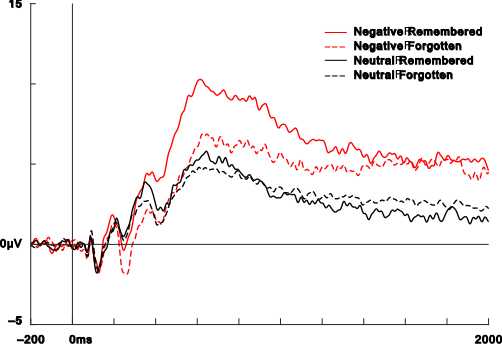
\includegraphics[keepaspectratio]{figures/media/image1.png}}

}

\end{figure}%

\begin{figure}

\caption{\label{fig-2}Early LPP topography and ERP differences}

\centering{

\pandocbounded{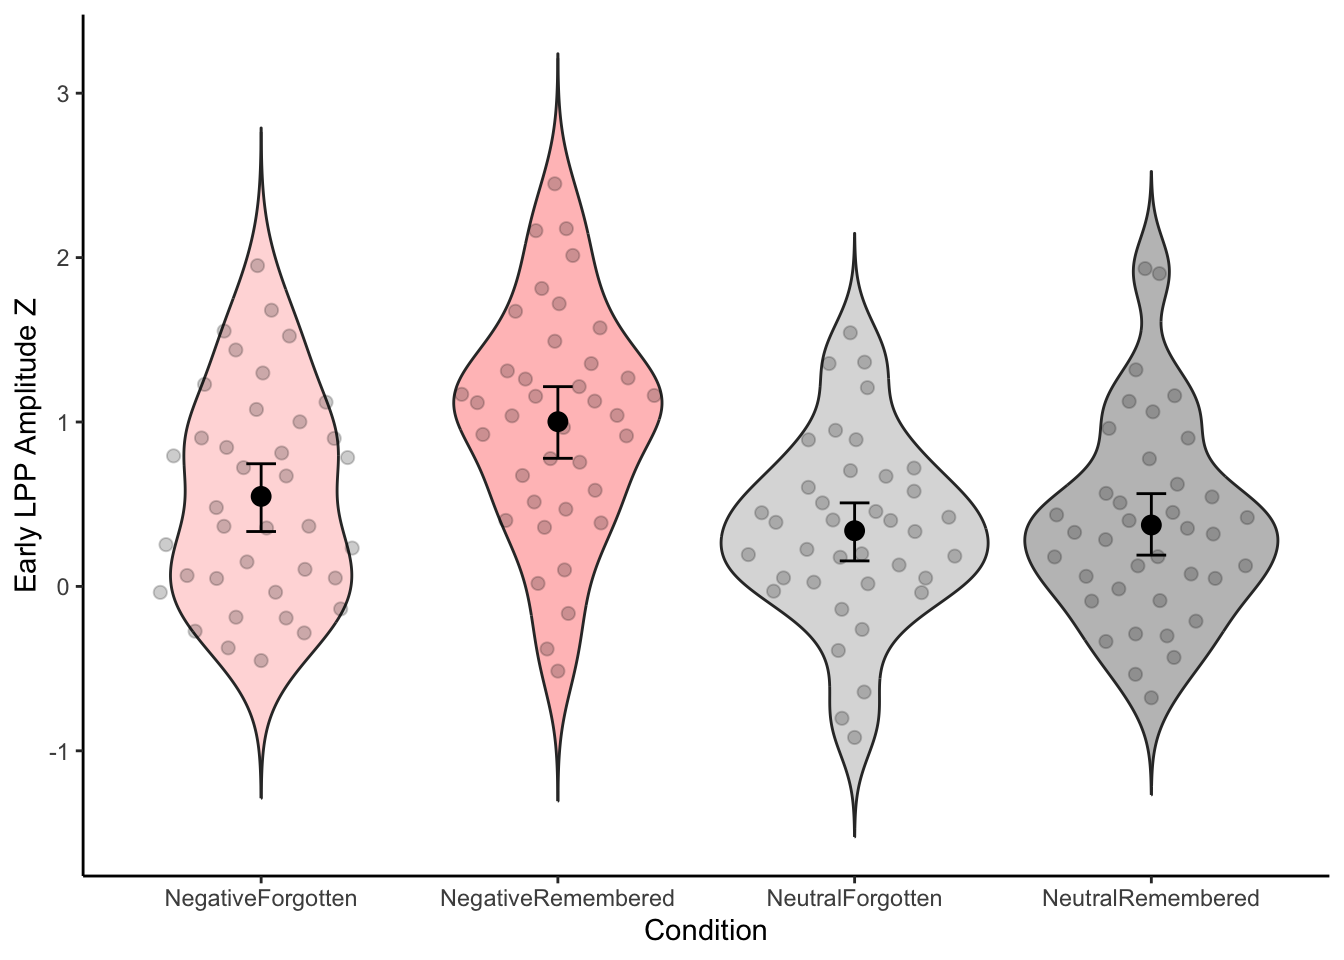
\includegraphics[keepaspectratio]{figures/media/image2.png}}

}

\end{figure}%

\begin{figure}

\caption{\label{fig-3}Late LPP ERP waveforms (1000--2000 ms)}

\centering{

\pandocbounded{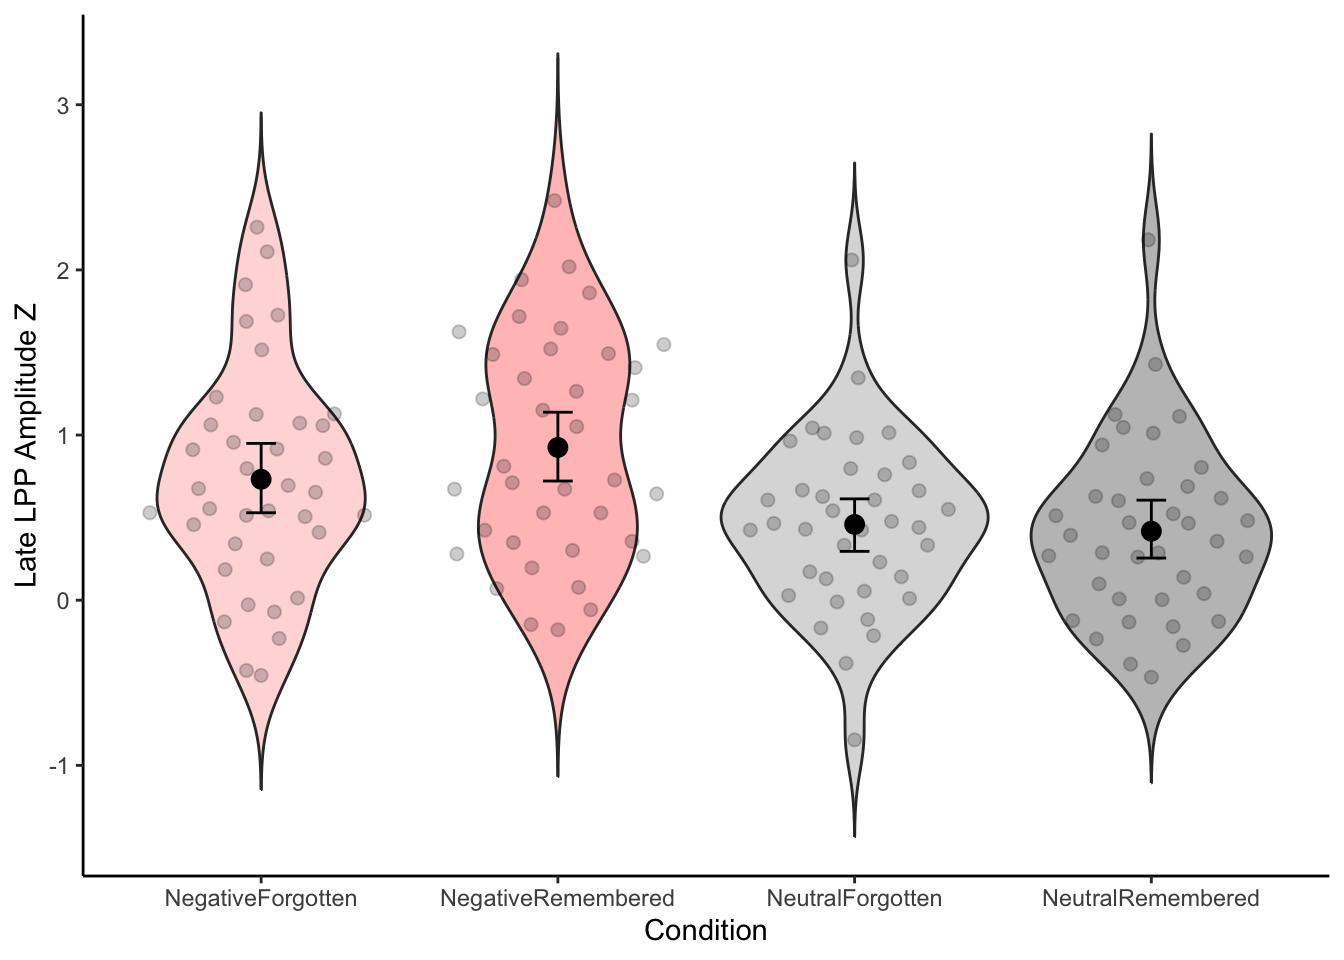
\includegraphics[keepaspectratio]{figures/media/image3.png}}

}

\end{figure}%

\paragraph{Global ERP Analysis.}\label{global-erp-analysis-1}

We first analysed the main effect of Emotion (Negative vs Neutral
trials) and found a positive cluster (\emph{p} \textless{} .001) which
was significant between approximately 380-2000ms with a widespread
distribution. In other words, there was an emotionally enhanced LPP
effect which roughly overlapped with the early and late time windows
analysed in the focal analysis.

Replicating the focal analysis, there was also a main effect of
subsequent memory with more positive ERPs for remembered compared to
forgotten trials (\emph{p} \textless{} .001) with a widespread spatial
distribution between around 210-1240ms.

In addition, there was an Emotion x Subsequent Memory interaction
between 360-1240ms (\emph{p} \textless{} .001) with a widespread
distribution, indicating that the negative items subsequent memory
effect was larger than the neutral items subsequent memory effect. In
addition, there was a borderline significant widespread cluster
(\emph{p} = .029) between 1240-1390ms. Follow-up cluster permutation
tests showed that for negative items, remembered items were related to
more positive going ERPs between 220-1420ms (\emph{p} \textless{} .001).
This effect was also widespread. In contrast, there was no significant
subsequent memory (all \emph{p}s \textgreater{} .19). ERP effect for
neutral items.

Overall, the global analysis replicated the focal analysis and shows
that these results hold up in more conservative tests with correction
for multiple comparisons. The analysis also shows that the time windows
and electrodes analysed in the focal analysis capture the maximum of the
LPP effects well in this data set.

\begin{figure}

\caption{\label{fig-4}Global ERP analysis: cluster summary}

\centering{

\pandocbounded{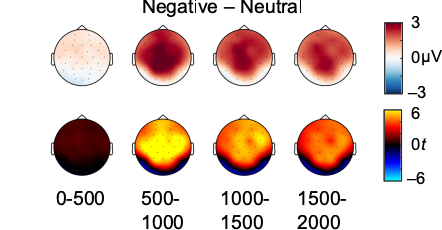
\includegraphics[keepaspectratio]{figures/media/image4.png}}

}

\end{figure}%

\begin{figure}

\caption{\label{fig-5}Global ERP analysis: detailed cluster results}

\centering{

\pandocbounded{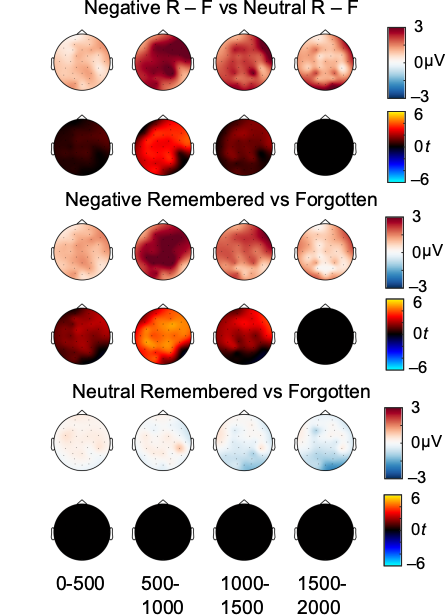
\includegraphics[keepaspectratio]{figures/media/image5.png}}

}

\end{figure}%

\paragraph{Bootstrap Reliability.}\label{bootstrap-reliability}

We next performed a bootstrap analysis to test if the emotional LPP
effect was reliable within subjects. This analysis showed that the early
LPP was reliable in 73.7\% of the participants while the late LPP effect
was reliable in 50\% of the participants.

\begin{figure}

\caption{\label{fig-6}Bootstrap reliability of the emotional LPP effect}

\centering{

\pandocbounded{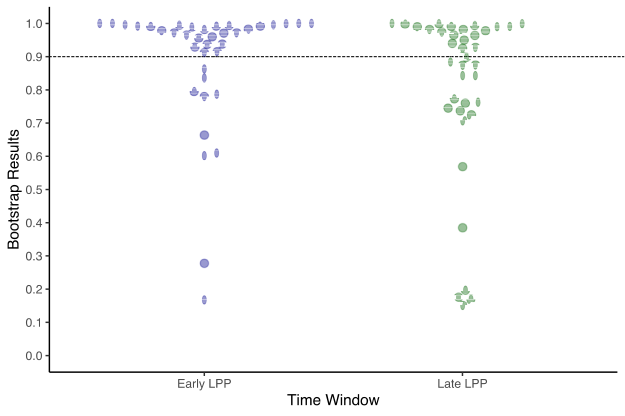
\includegraphics[keepaspectratio]{figures/media/image6.png}}

}

\end{figure}%

\paragraph{LPP and Emotion Enhanced
Memory.}\label{lpp-and-emotion-enhanced-memory}

To be useful for the purpose of model constraint the LPP will need to
correlate with memory performance. We first investigated if the
emotionally enhanced LPP amplitude (negative minus neutral items)
correlated with emotionally enhanced memory (negative minus neutral
items) between subjects. Surprisingly, the Bayesian Pearson correlation
showed moderate evidence for no correlation for both the early time
window (\emph{r} = --.018, BF\textsubscript{01} = 4.925) and the late
time window (\emph{r} = --.028, BF\textsubscript{01} = 4.885).

Next, we investigated the correlation between emotion enhanced LPP
amplitude and emotion enhanced memory within subjects. For each subject,
we correlated the emotion enhanced LPP with the emotion enhanced memory
across the 9 lists. We then calculated the average correlation
coefficient for each subject and tested it against zero using a
one-sample Bayesian \emph{t}-test. There was moderate support for no
correlation in both the early time window (\emph{t}(37) = --.26,
\emph{p} = .795, BF\textsubscript{01} = 7.658) and the late time window
(\emph{t}(37) = --1.26, \emph{p} = .215, BF\textsubscript{01} = 3.698).

Finally, we conducted binomial generalized mixed effects models to test
if Emotion and LPP amplitude predicted memory separately for the two
time windows. In the early time window, there was a main effect of
Emotion (\(\beta\) = .21, \(\chi^2\)(1) = 22.68, \emph{p} \textless{}
.001), a main effect of LPP (\(\beta\) = .08, \(\chi^2\)(1) = 18.87,
\emph{p} \textless{} .001) and an Emotion x LPP interaction (\(\beta\) =
.06, \(\chi^2\)(1) = 11.20, \emph{p} \textless{} .001). The interaction
was followed-up by running the same analysis separately for negative and
neutral items. For negative items, there was a significant positive
relationship between early LPP amplitude and memory (\(\beta\) = .14,
\(\chi^2\)(1) = 25.43, \emph{p} \textless{} .001). In contrast, there
was no significant relationship between early LPP amplitude and memory
for neutral items (\(\beta\) = .01, \(\chi^2\)(1) = .48, \emph{p} =
.488). In the late time window, there was a main effect of Emotion
(\(\beta\) = .23, \(\chi^2\)(1) = 66.58, \emph{p} \textless{} .001),
showing once again that memory was higher for negative than neutral
items, but importantly there was neither a main effect of LPP amplitude
(\(\beta\) = .02, \(\chi^2\)(1) = 1.98, \emph{p} = .160) nor any
interaction between Emotion and LPP amplitude (\(\beta\) = .02,
\(\chi^2\)(1) = 2.44, \emph{p} = .118).

In sum, the analyses show that the early LPP is more reliable and
related to emotion-enhanced memory on a single-trial level. Based on
this, we will use single-trial data from the early LPP time window to
constrain the eCMR model.

\begin{figure}

\caption{\label{fig-7}Between-subjects LPP--memory correlation overview}

\centering{

\pandocbounded{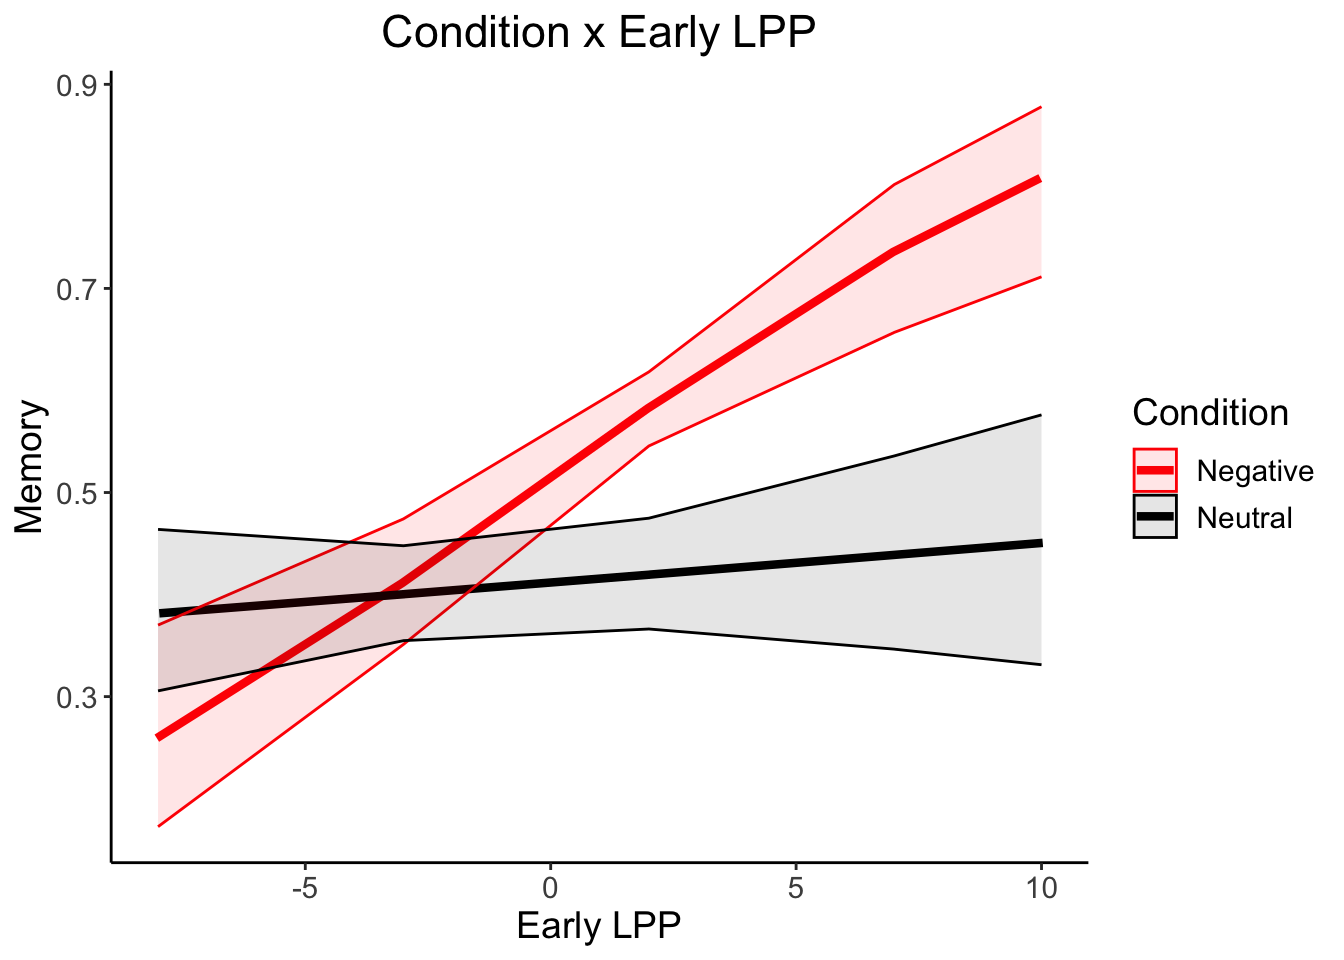
\includegraphics[keepaspectratio]{figures/media/image7.png}}

}

\end{figure}%

\begin{figure}

\caption{\label{fig-8}Early LPP between-subjects scatter plot}

\centering{

\pandocbounded{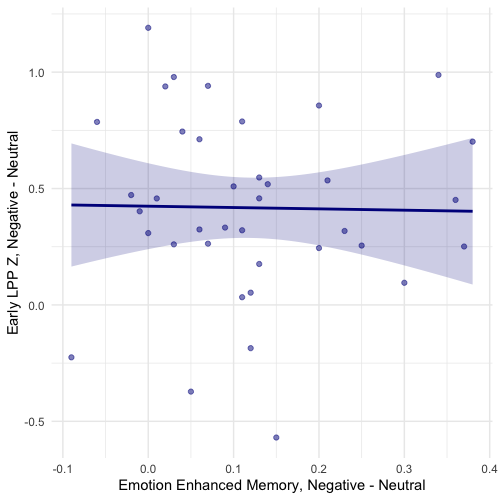
\includegraphics[keepaspectratio]{figures/media/image8.png}}

}

\end{figure}%

\begin{figure}

\caption{\label{fig-9}Late LPP between-subjects scatter plot}

\centering{

\pandocbounded{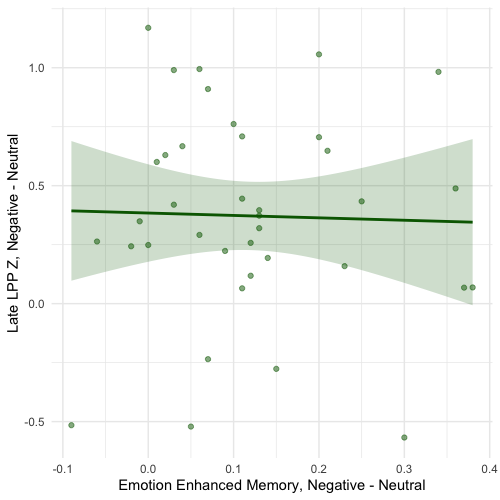
\includegraphics[keepaspectratio]{figures/media/image9.png}}

}

\end{figure}%

\begin{figure}

\caption{\label{fig-10}Within-subjects LPP--memory correlation}

\centering{

\pandocbounded{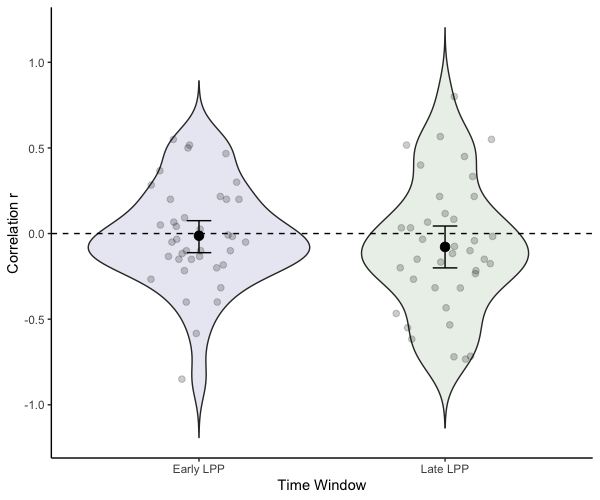
\includegraphics[keepaspectratio]{figures/media/image10.png}}

}

\end{figure}%

\subsubsection{eCMR Model Comparison}\label{ecmr-model-comparison}

Table~\ref{tbl-comparison} summarizes the four-model comparison. We
first tested whether eCMR's emotional context layer and
encoding-strength modulation improve prediction over CMR's
temporal-context baseline. eCMR achieved strictly lower negative
log-likelihood (NLL) than CMR for 89.5\% of participants. By AIC, this
advantage was reliable, with mean \(\Delta\)AIC (CMR \(-\) eCMR) = 4.06
{[}1.36, 6.77{]} and the CI excluding zero. Bayesian model selection
assigned CMR an exceedance probability of .009 and an expected frequency
of .175 (Table~\ref{tbl-comparison}), confirming that the dual-context
mechanism captures meaningful structure in emotional recall beyond
temporal dynamics alone.

We next asked whether the LPP alone can account for emotional memory
effects. CMR+LPP achieved lower NLL than CMR for 65.8\% of participants,
but this improvement did not offset the AIC penalty for the additional
parameter: mean \(\Delta\)AIC (CMR \(-\) CMR+LPP) = 0.33 {[}\(-0.77\),
1.44{]}, with the CI including zero. BMS assigned CMR+LPP an expected
frequency of .089 and an exceedance probability below .001
(Table~\ref{tbl-comparison}). The LPP carries some information about
which items will be recalled, but too little per subject for one
additional parameter to clear the AIC bar.

The critical comparison pits the LPP against category labels at equal
parameter cost (\(k = 10\)). eCMR achieved lower NLL than CMR+LPP for
68.4\% of participants. Mean \(\Delta\)AIC (CMR+LPP \(-\) eCMR) = 3.73
{[}1.23, 6.22{]} and the CI excludes zero; the median \(\Delta\)AIC =
1.52 {[}0.18, 2.86{]} also excludes zero. At equal parameter cost,
category labels embedded in the emotional context architecture captured
substantially more variance than trial-level LPP operating through the
temporal pathway.

Turning to the LPP constraint, LPP-eCMR achieved strictly lower NLL than
eCMR for 73.7\% of participants, with the remainder tied after nesting
flooring. By aggregate AIC weights, LPP-eCMR was strongly favored (\(w\)
= .997 vs .003; Table~\ref{tbl-comparison}), and Bayesian model
selection also favored LPP-eCMR (exceedance probability = .721 vs .269).

This aggregate advantage was not uniform across individuals. The mean
per-subject \(\Delta\)AIC (eCMR \(-\) LPP-eCMR) was 0.30 {[}\(-0.70\),
1.29{]}, consistent with practical equivalence, and the median was
\(-1.21\) {[}\(-2.36\), \(-0.06\){]}, indicating that the typical
participant's NLL improvement did not offset the penalty for the
additional parameter. Protected exceedance probabilities confirmed this
heterogeneity, remaining at chance (.250 each). Together, these results
indicate that a subset of participants benefit substantially from the
LPP term --- enough to dominate the aggregate --- while for the
remainder the LPP adds little beyond what category labels already
capture.

In sum, the emotional context architecture is essential (CMR \(<\)
eCMR), the LPP cannot replace it (CMR+LPP \(\approx\) CMR \(\ll\) eCMR),
and supplementing category labels with the LPP yields a genuine
aggregate fit advantage concentrated among participants for whom the LPP
carries the most information about subsequent recall.

\begin{table}

{\caption{{Model comparison summary. \(k\) = free parameters; NLL =
negative log-likelihood (mean \(\pm\) SE across 38 participants);
AIC\(w\) = aggregate AIC weight; BMS \(r\) = expected model frequency;
BMS XP = exceedance probability.}{\label{tbl-comparison}}}
\vspace{-20pt}}

\begin{longtable}[]{@{}
  >{\raggedright\arraybackslash}p{(\linewidth - 10\tabcolsep) * \real{0.1515}}
  >{\centering\arraybackslash}p{(\linewidth - 10\tabcolsep) * \real{0.0758}}
  >{\centering\arraybackslash}p{(\linewidth - 10\tabcolsep) * \real{0.3182}}
  >{\centering\arraybackslash}p{(\linewidth - 10\tabcolsep) * \real{0.1970}}
  >{\centering\arraybackslash}p{(\linewidth - 10\tabcolsep) * \real{0.1364}}
  >{\centering\arraybackslash}p{(\linewidth - 10\tabcolsep) * \real{0.1212}}@{}}
\toprule\noalign{}
\begin{minipage}[b]{\linewidth}\raggedright
Model
\end{minipage} & \begin{minipage}[b]{\linewidth}\centering
\(k\)
\end{minipage} & \begin{minipage}[b]{\linewidth}\centering
Mean NLL (\(\pm\) SE)
\end{minipage} & \begin{minipage}[b]{\linewidth}\centering
AIC\(w\)
\end{minipage} & \begin{minipage}[b]{\linewidth}\centering
BMS \(r\)
\end{minipage} & \begin{minipage}[b]{\linewidth}\centering
BMS XP
\end{minipage} \\
\midrule\noalign{}
\endhead
\bottomrule\noalign{}
\endlastfoot
CMR & 9 & 215.01 \(\pm\) 15.63 & \(\approx\) 0 & .175 & .009 \\
CMR+LPP & 10 & 213.84 \(\pm\) 15.73 & \(\approx\) 0 & .089 &
\textless.001 \\
eCMR & 10 & 211.98 \(\pm\) 16.31 & .003 & .328 & .269 \\
LPP-eCMR & 11 & 210.83 \(\pm\) 16.46 & .997 & .407 & .721 \\
\end{longtable}

\end{table}

We assessed qualitative adequacy with two benchmark diagnostics
(Figure~\ref{fig-catspc}; Figure~\ref{fig-lpp-recall}). The first
targets the emotional enhancement of memory established in the
Behavioural Results. Category-specific serial position curves
(Figure~\ref{fig-catspc}) show that CMR, which lacks an emotional
context layer, predicts nearly identical recall for negative and neutral
items. CMR+LPP produces a faint separation because LPP amplitude
correlates weakly with emotional category, but the effect is far weaker
than what the emotional context architecture achieves. Both eCMR and
LPP-eCMR reproduce the empirical separation: their shared emotional
context ensures that negative items promote one another's recall,
lifting the negative SPC above the neutral baseline.

A second diagnostic targets the LPP--recall link established in the EEG
Results. Despite aggregate AIC indistinguishability between eCMR and
LPP-eCMR, the models make qualitatively different predictions about an
untrained summary statistic. Empirically, recalled emotional items had
higher Early LPP amplitudes than unrecalled emotional items; no such
difference existed for neutral items, consistent with the GLMM. eCMR
cannot reproduce this pattern: it assigns identical encoding strength to
all emotional items regardless of their LPP amplitude, so simulated LPP
distributions for recalled and unrecalled emotional items overlap. Both
CMR+LPP and LPP-eCMR reproduce the separation, since both use LPP to
modulate encoding strength. Higher LPP leads to stronger encoding and
higher recall probability (Figure~\ref{fig-lpp-recall}). The critical
difference is that only LPP-eCMR also captures the category-level recall
structure visible in the SPC diagnostic. This outcome reflects genuine
generalization since the models are fit to set likelihood, not to the
recalled-versus-unrecalled LPP statistic. LPP-eCMR captures a
mechanistic link (LPP \(\rightarrow\) encoding strength \(\rightarrow\)
recall probability) that produces the observed neural-behavioral
association as a consequence of its architecture, while also reproducing
the categorical emotional memory advantage.

The LPP thus carries real information about emotional encoding strength,
as demonstrated by CMR+LPP and LPP-eCMR reproducing the LPP-by-recall
pattern that CMR and eCMR cannot. However, the LPP alone is not a
substitute for category labels: it cannot reproduce the categorical
recall advantage, and its per-subject signal is small relative to the
AIC cost of one parameter. The value of incorporating trial-level neural
measures is not in replacing existing model structure or uniformly
improving fit. It is in characterizing which individuals benefit from
the neural constraint and in generating mechanistic predictions that
were not used as fitting targets.

\begin{figure}

\caption{\label{fig-catspc}Category-specific serial position curves. Top
row: empirical data, CMR, CMR+LPP. Bottom row: eCMR, LPP-eCMR. CMR
predicts nearly identical curves; CMR+LPP produces a faint separation
via indirect LPP--category correlation; eCMR and LPP-eCMR reproduce the
full negative-above-neutral separation.}

\begin{minipage}{0.33\linewidth}
\pandocbounded{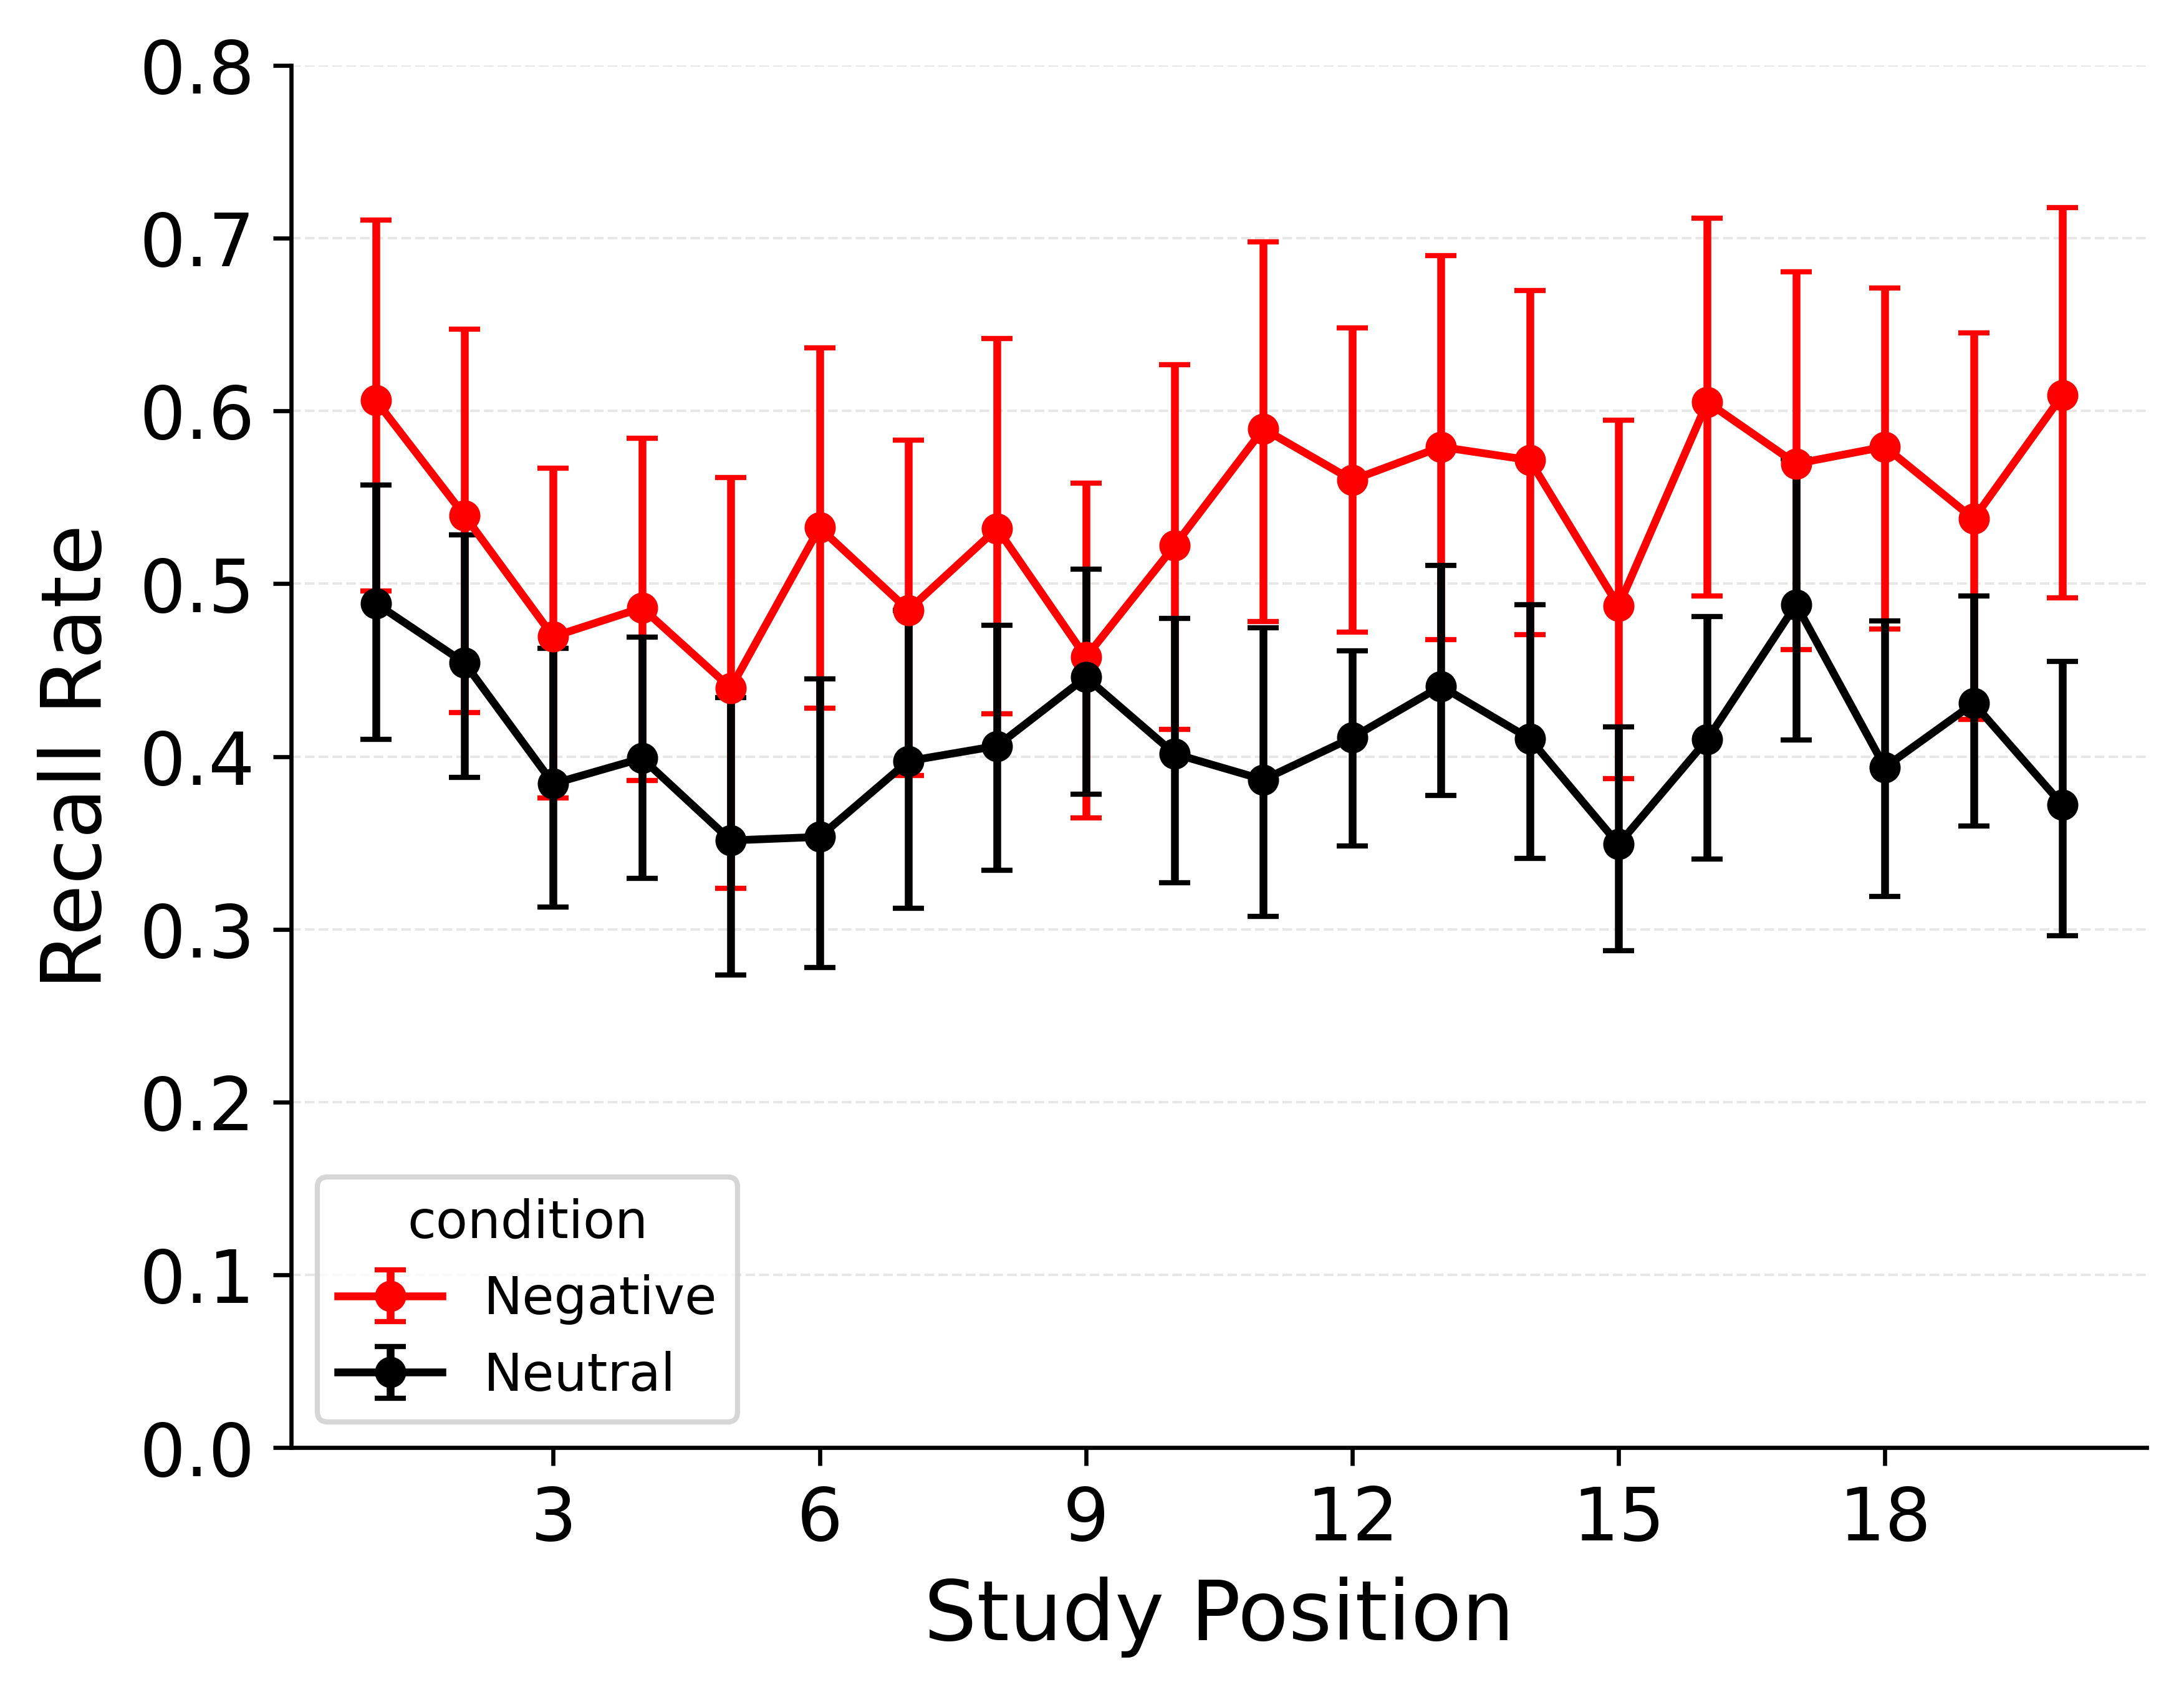
\includegraphics[keepaspectratio]{figures/analyses/reference_catspc.png}}\end{minipage}%
%
\begin{minipage}{0.33\linewidth}
\pandocbounded{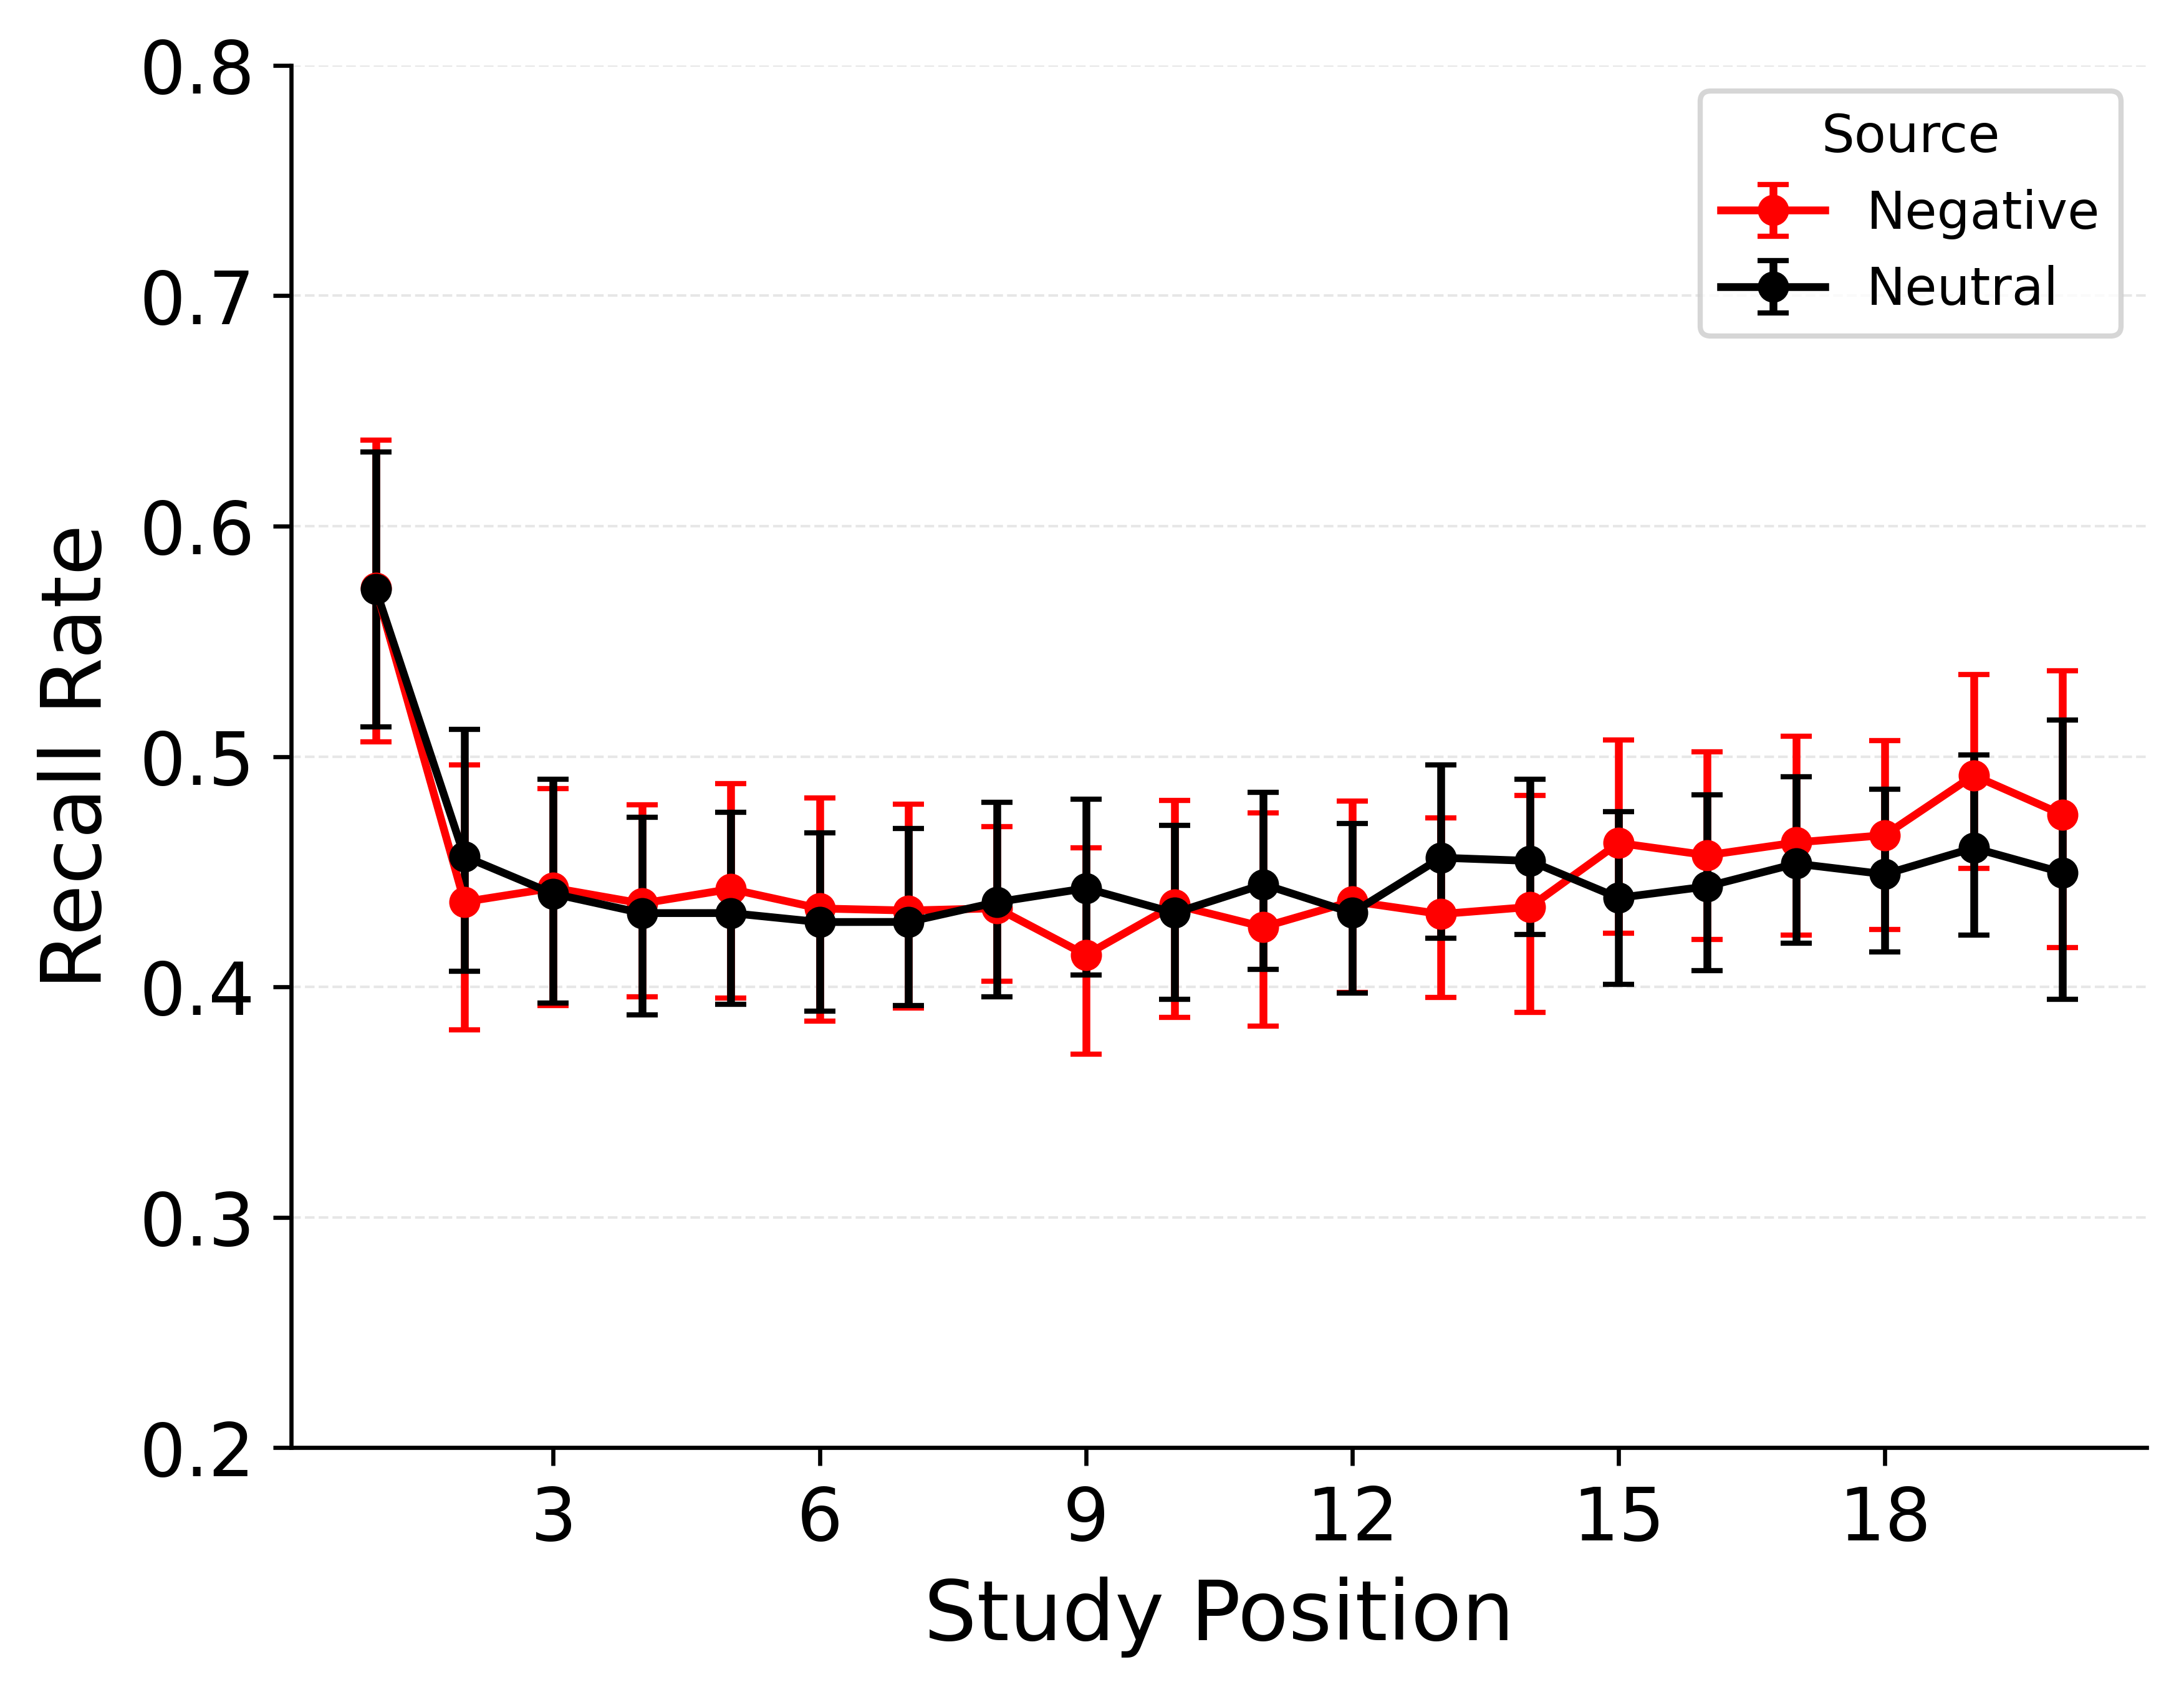
\includegraphics[keepaspectratio]{figures/fitting/TalmiEEG_WeirdCMRNoStop_50_set_likelihood_fixed_term_best_of_3_cat_spc.png}}\end{minipage}%
%
\begin{minipage}{0.33\linewidth}
\pandocbounded{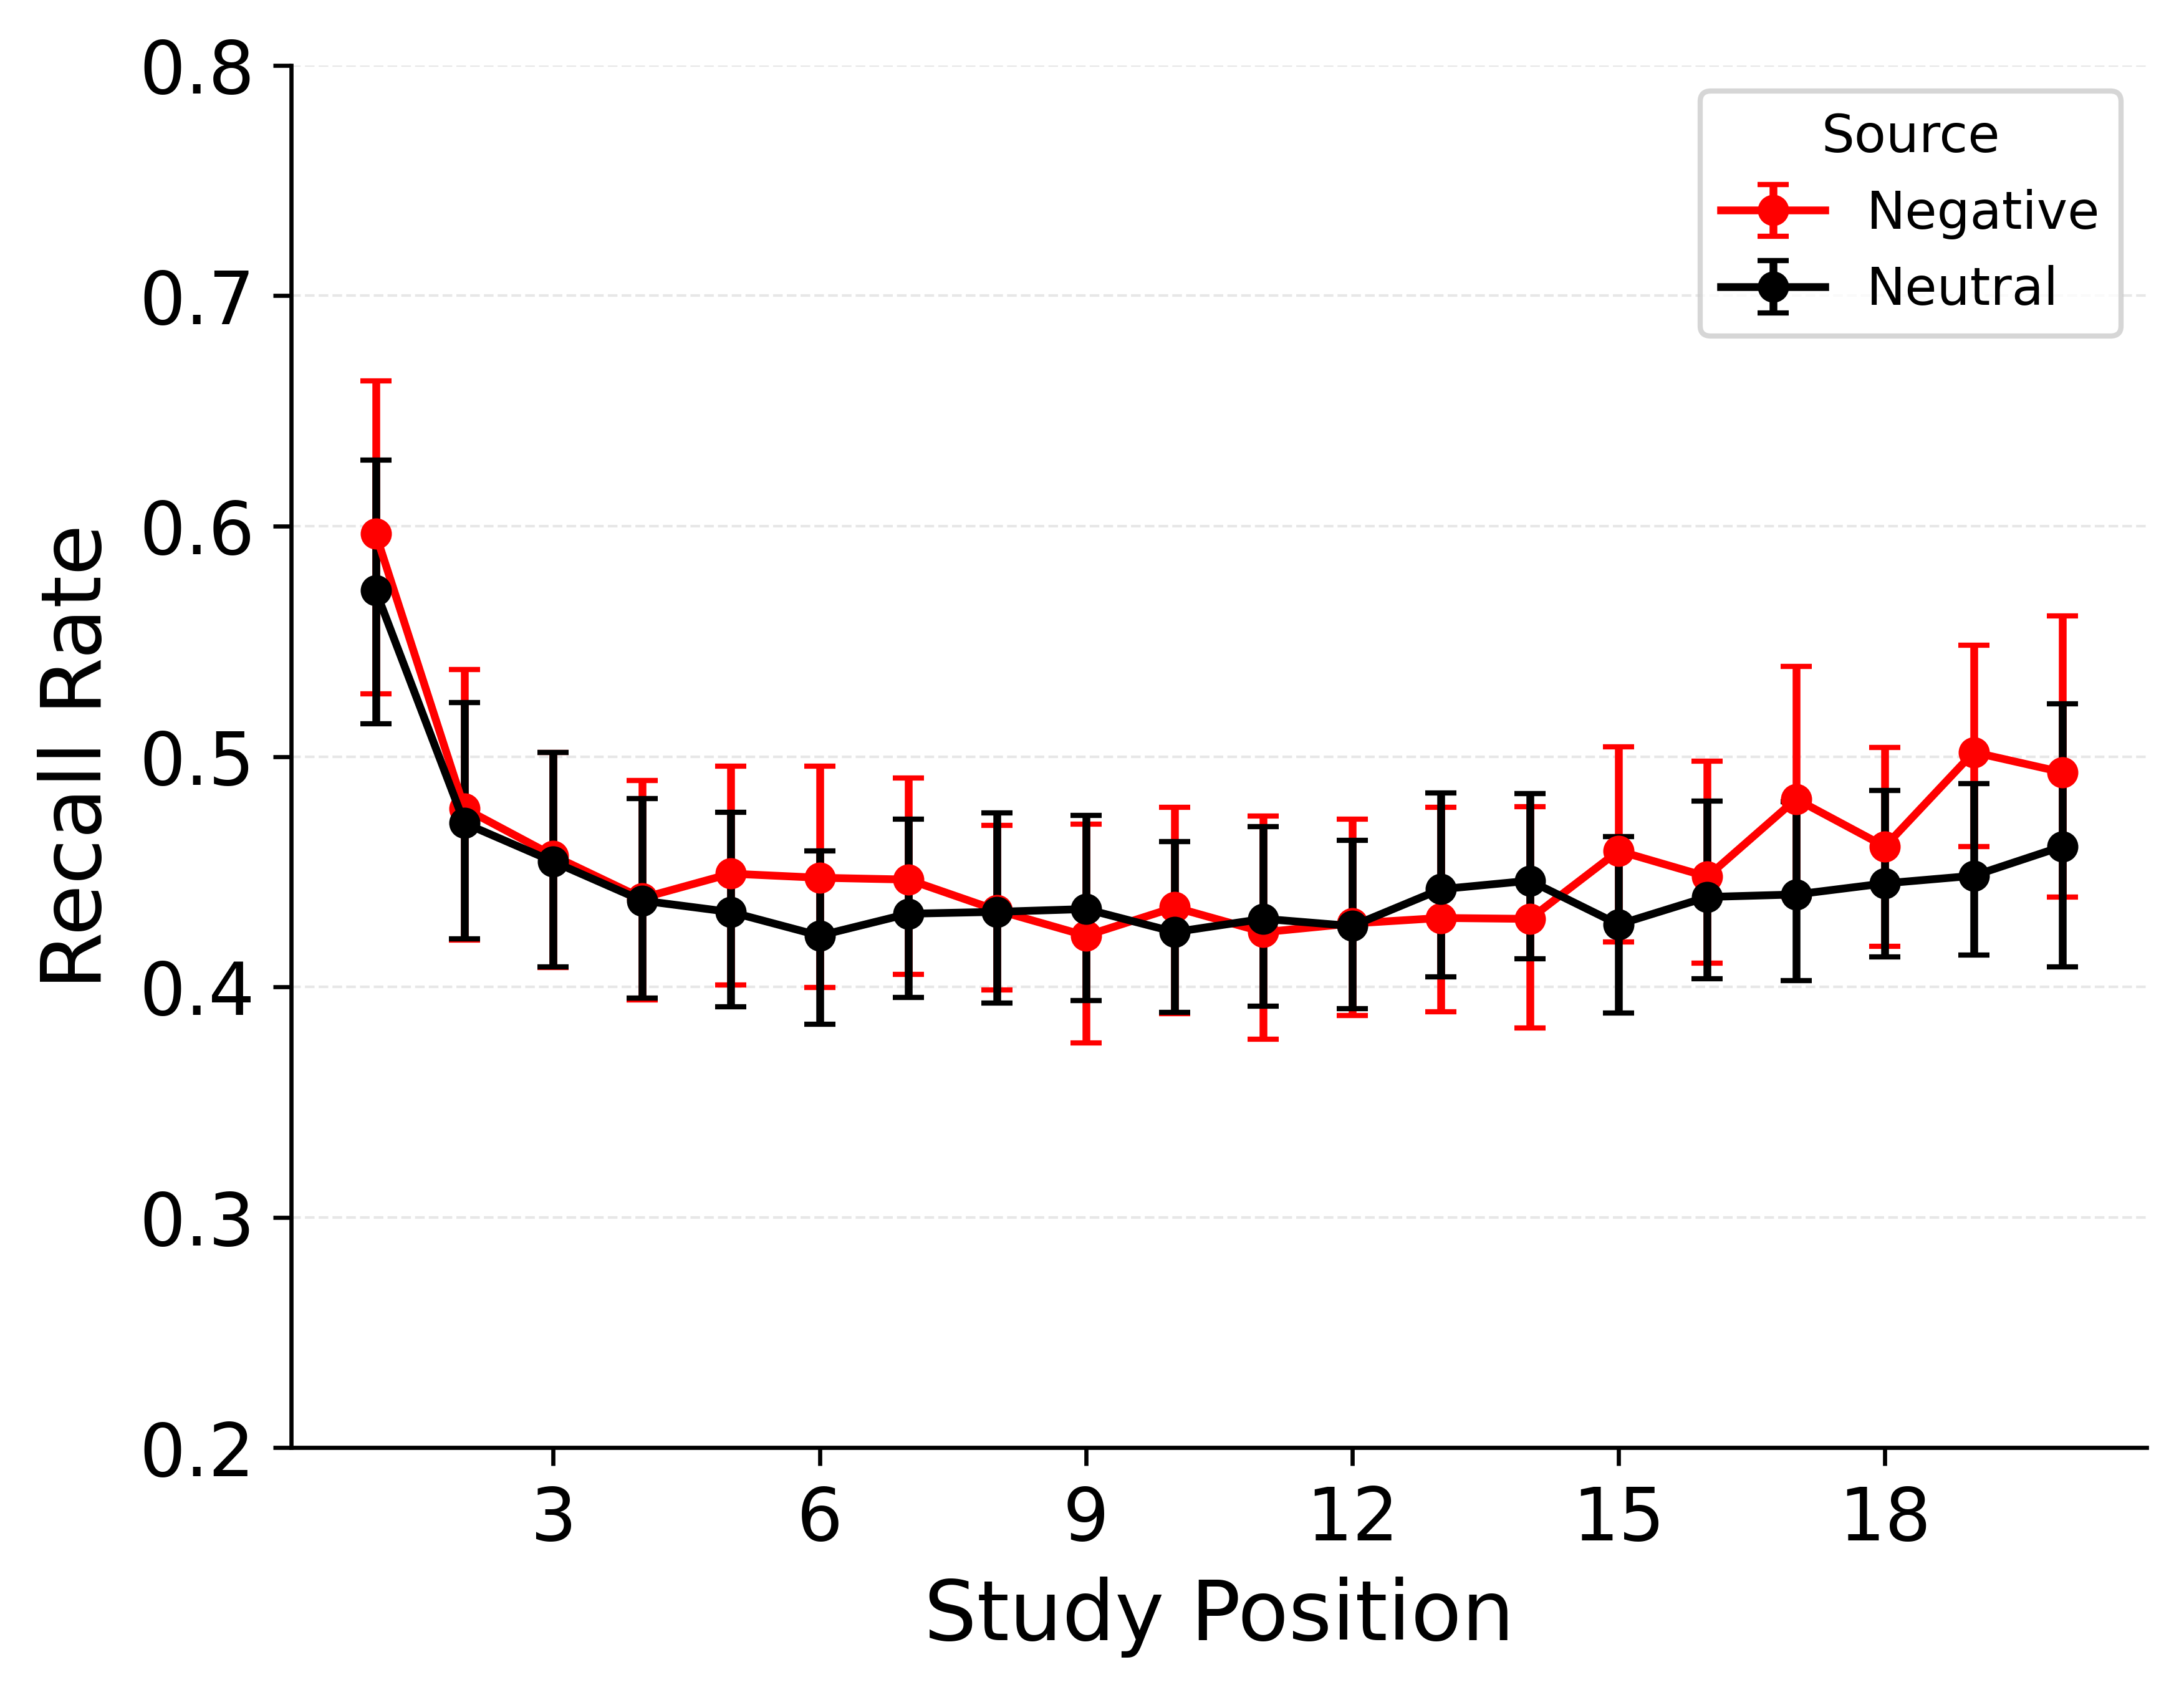
\includegraphics[keepaspectratio]{figures/fitting/TalmiEEG_EEGLPPParsimonious_50_set_likelihood_fixed_term_best_of_3_cat_spc.png}}\end{minipage}%
\newline
\begin{minipage}{0.33\linewidth}
\pandocbounded{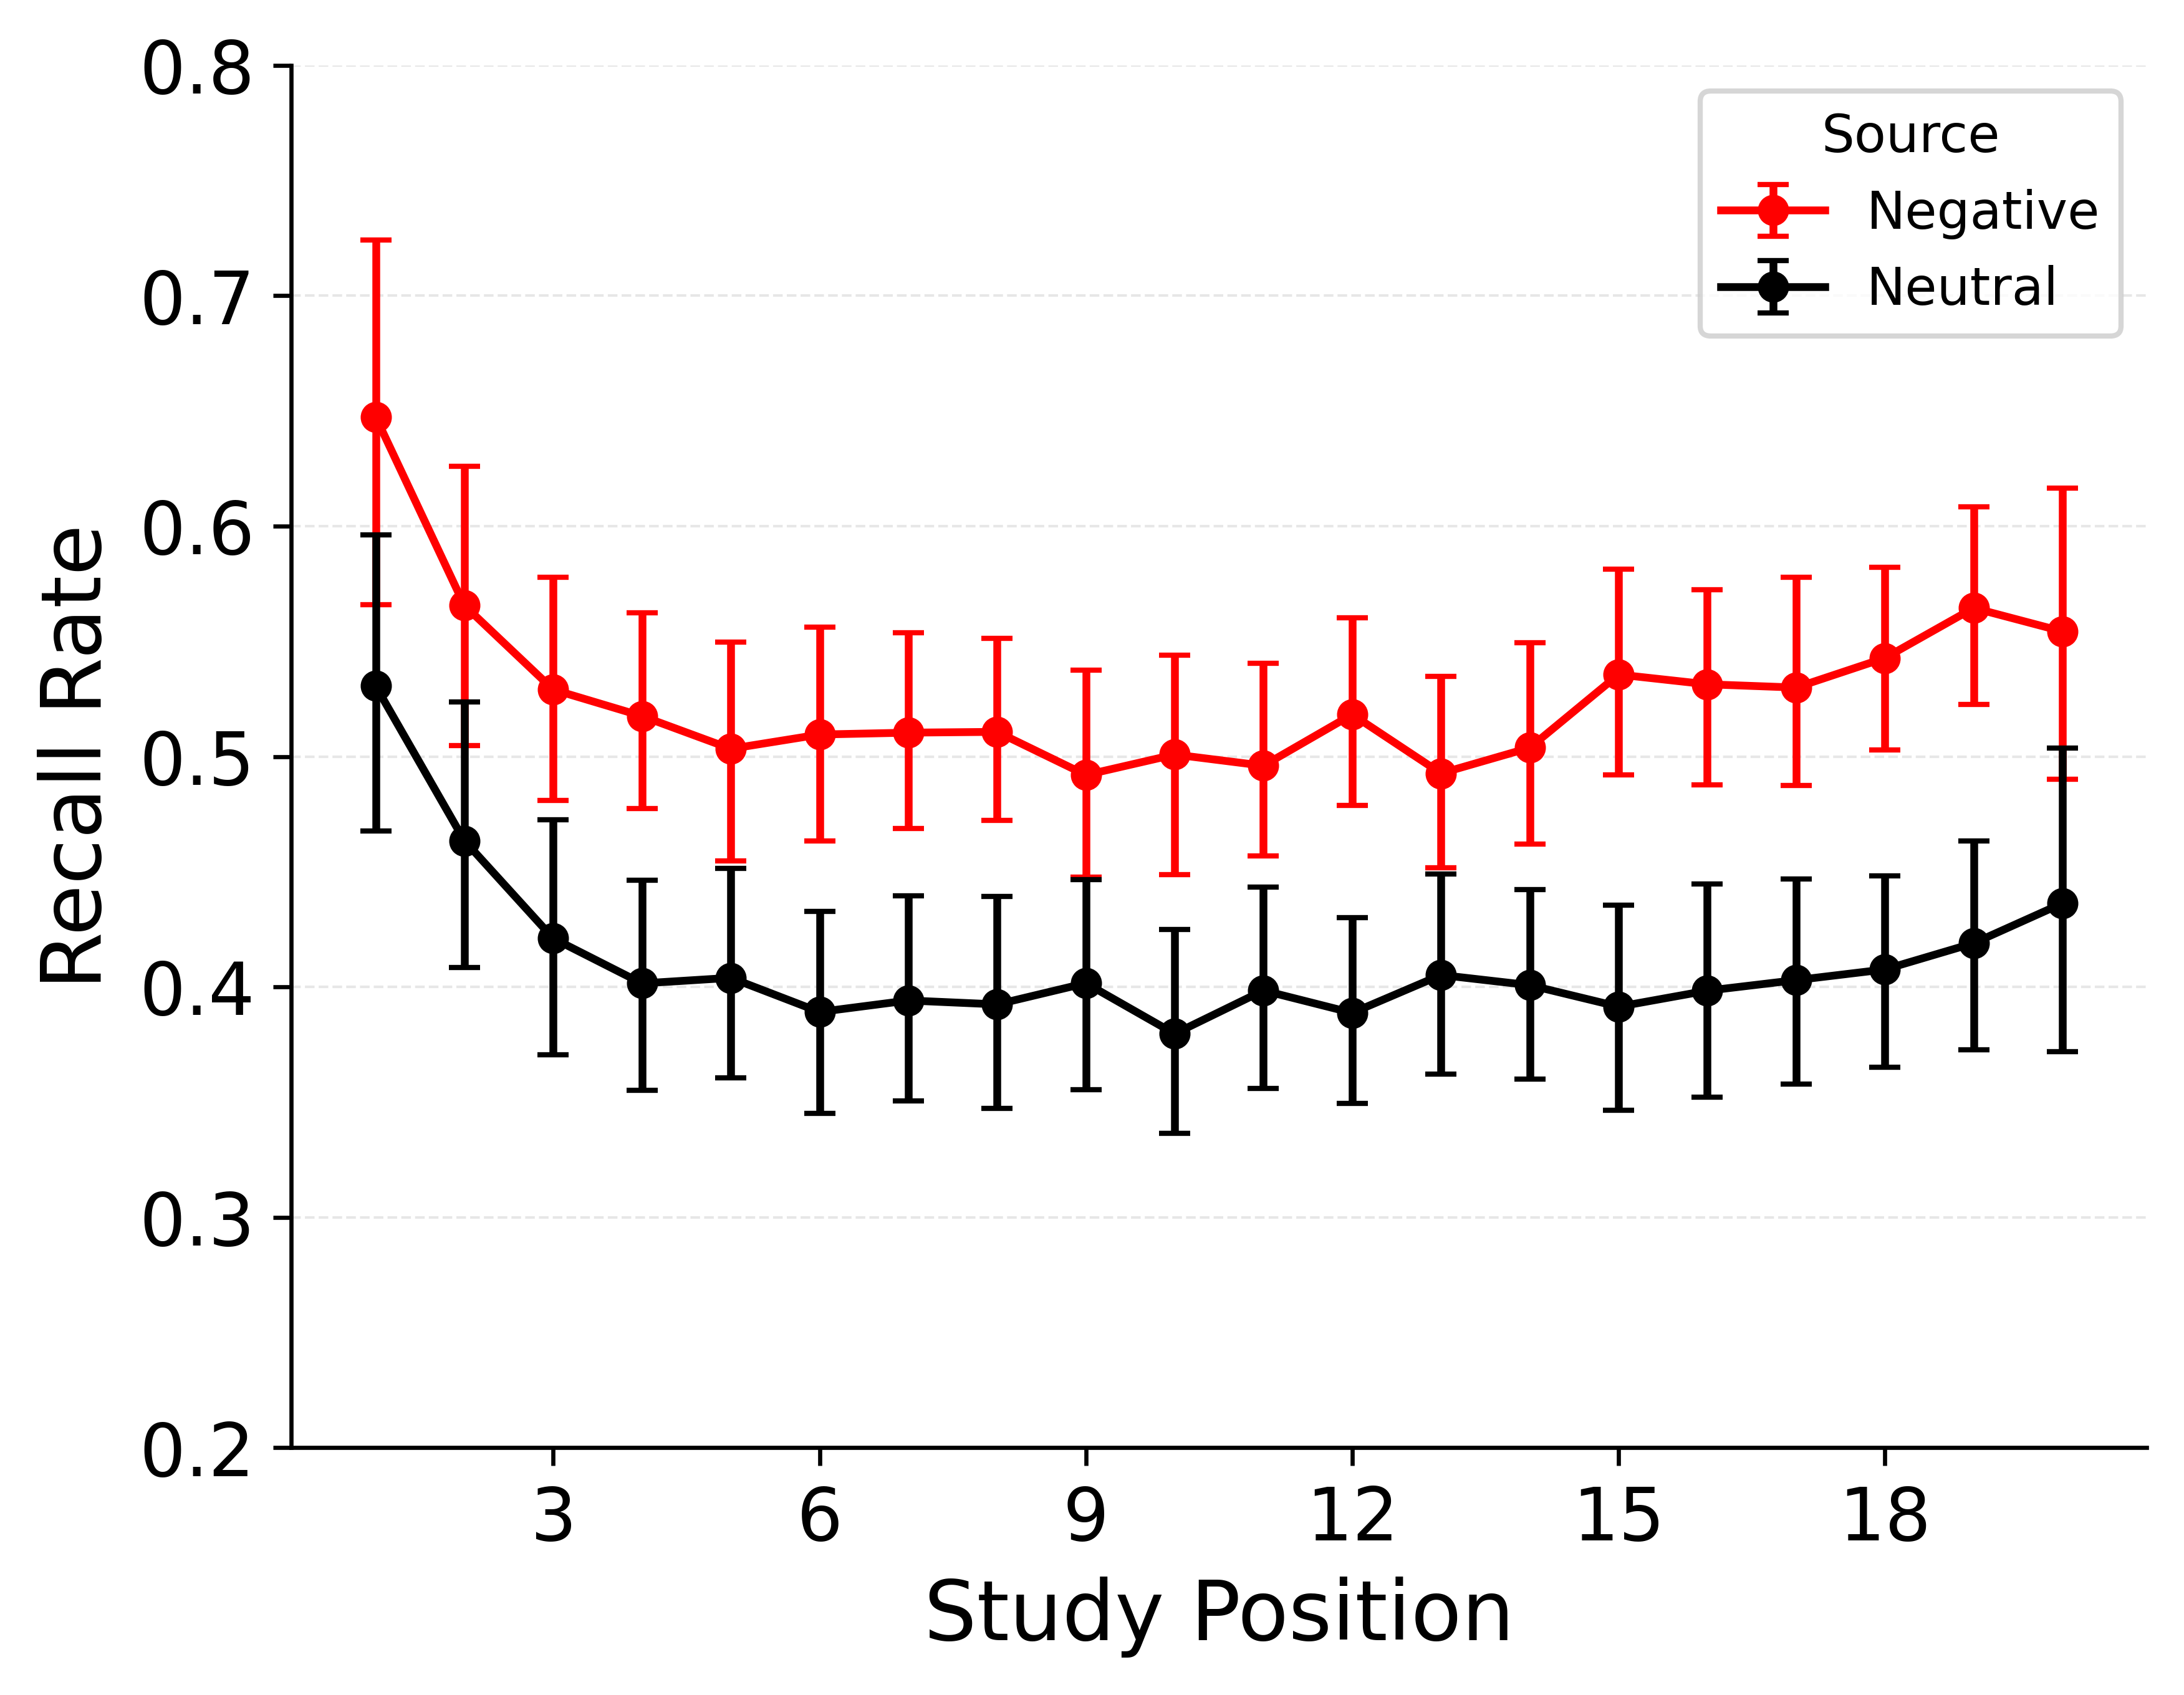
\includegraphics[keepaspectratio]{figures/fitting/TalmiEEG_eCMREmotionOnly_20260309_50_set_likelihood_best_of_3_cat_spc.png}}\end{minipage}%
%
\begin{minipage}{0.33\linewidth}
\pandocbounded{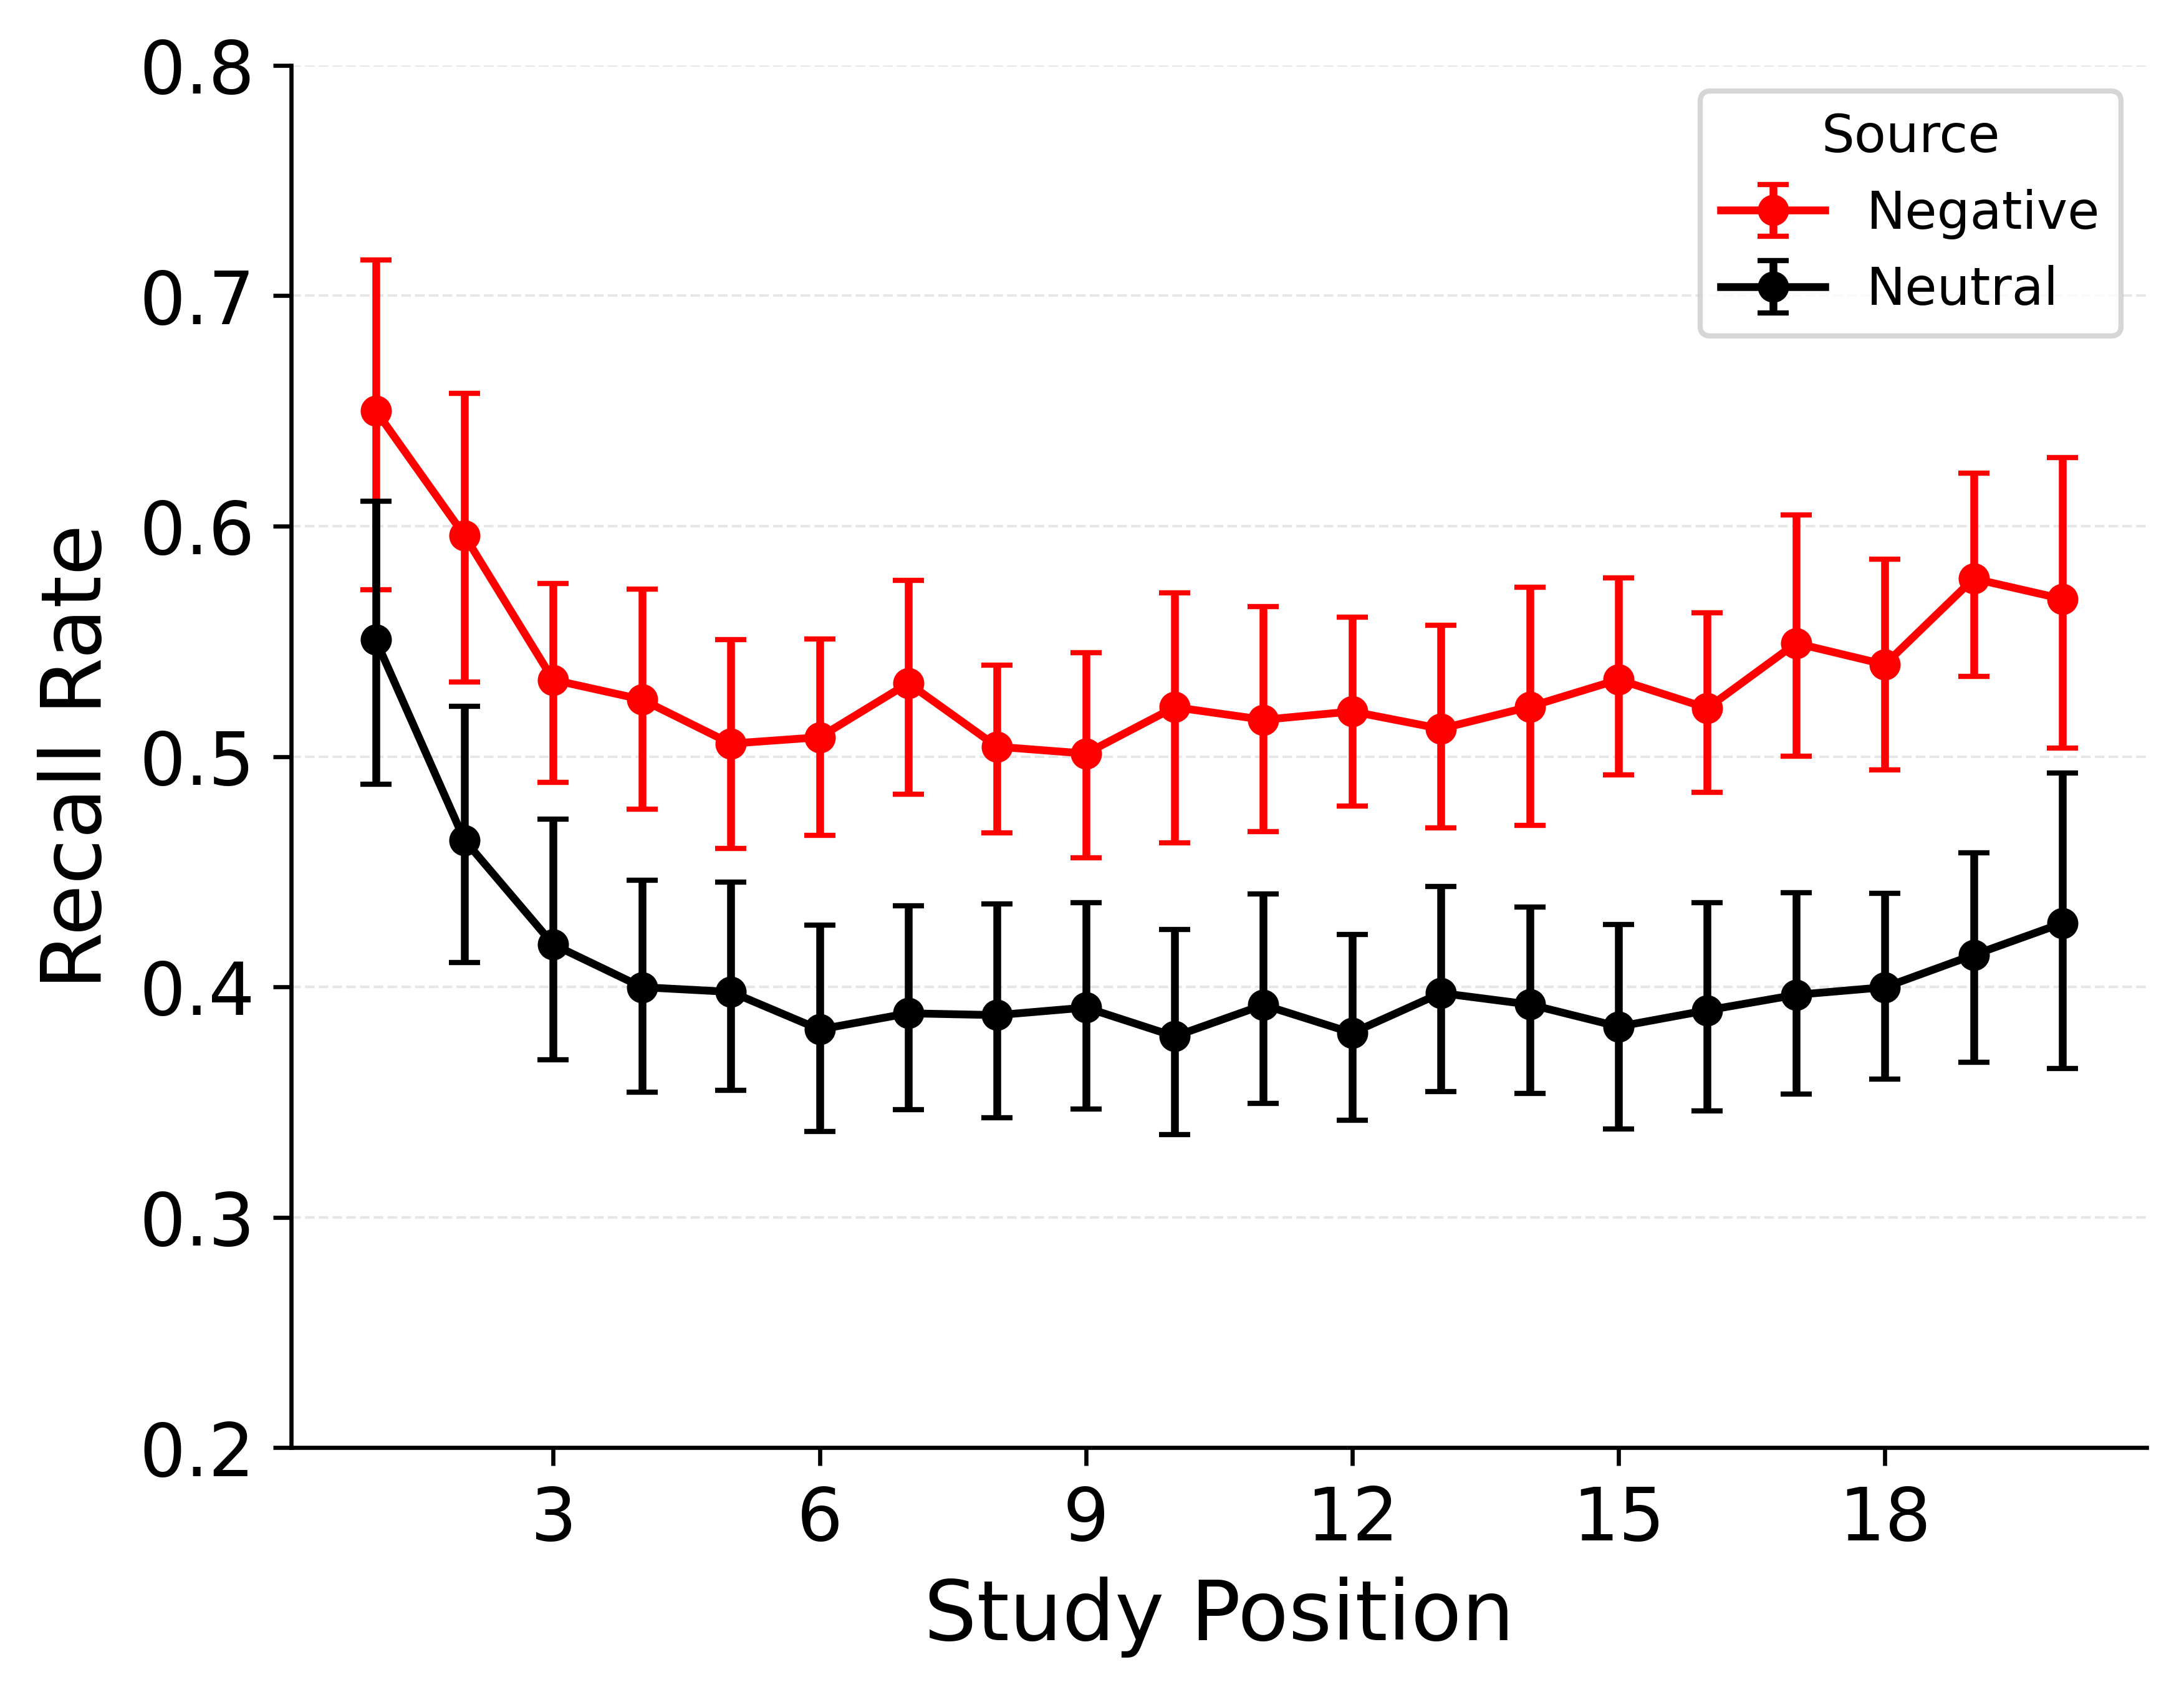
\includegraphics[keepaspectratio]{figures/fitting/TalmiEEG_eCMREmotionTimesLPP_20260309_50_set_likelihood_best_of_3_cat_spc.png}}\end{minipage}%

\end{figure}%

\begin{figure}

\caption{\label{fig-lpp-recall}Early LPP amplitude by recall status for
negative items. Top row: empirical data, CMR, CMR+LPP. Bottom row: eCMR,
LPP-eCMR. CMR+LPP and LPP-eCMR both reproduce the recalled/unrecalled
separation; CMR and eCMR cannot.}

\begin{minipage}{0.33\linewidth}
\pandocbounded{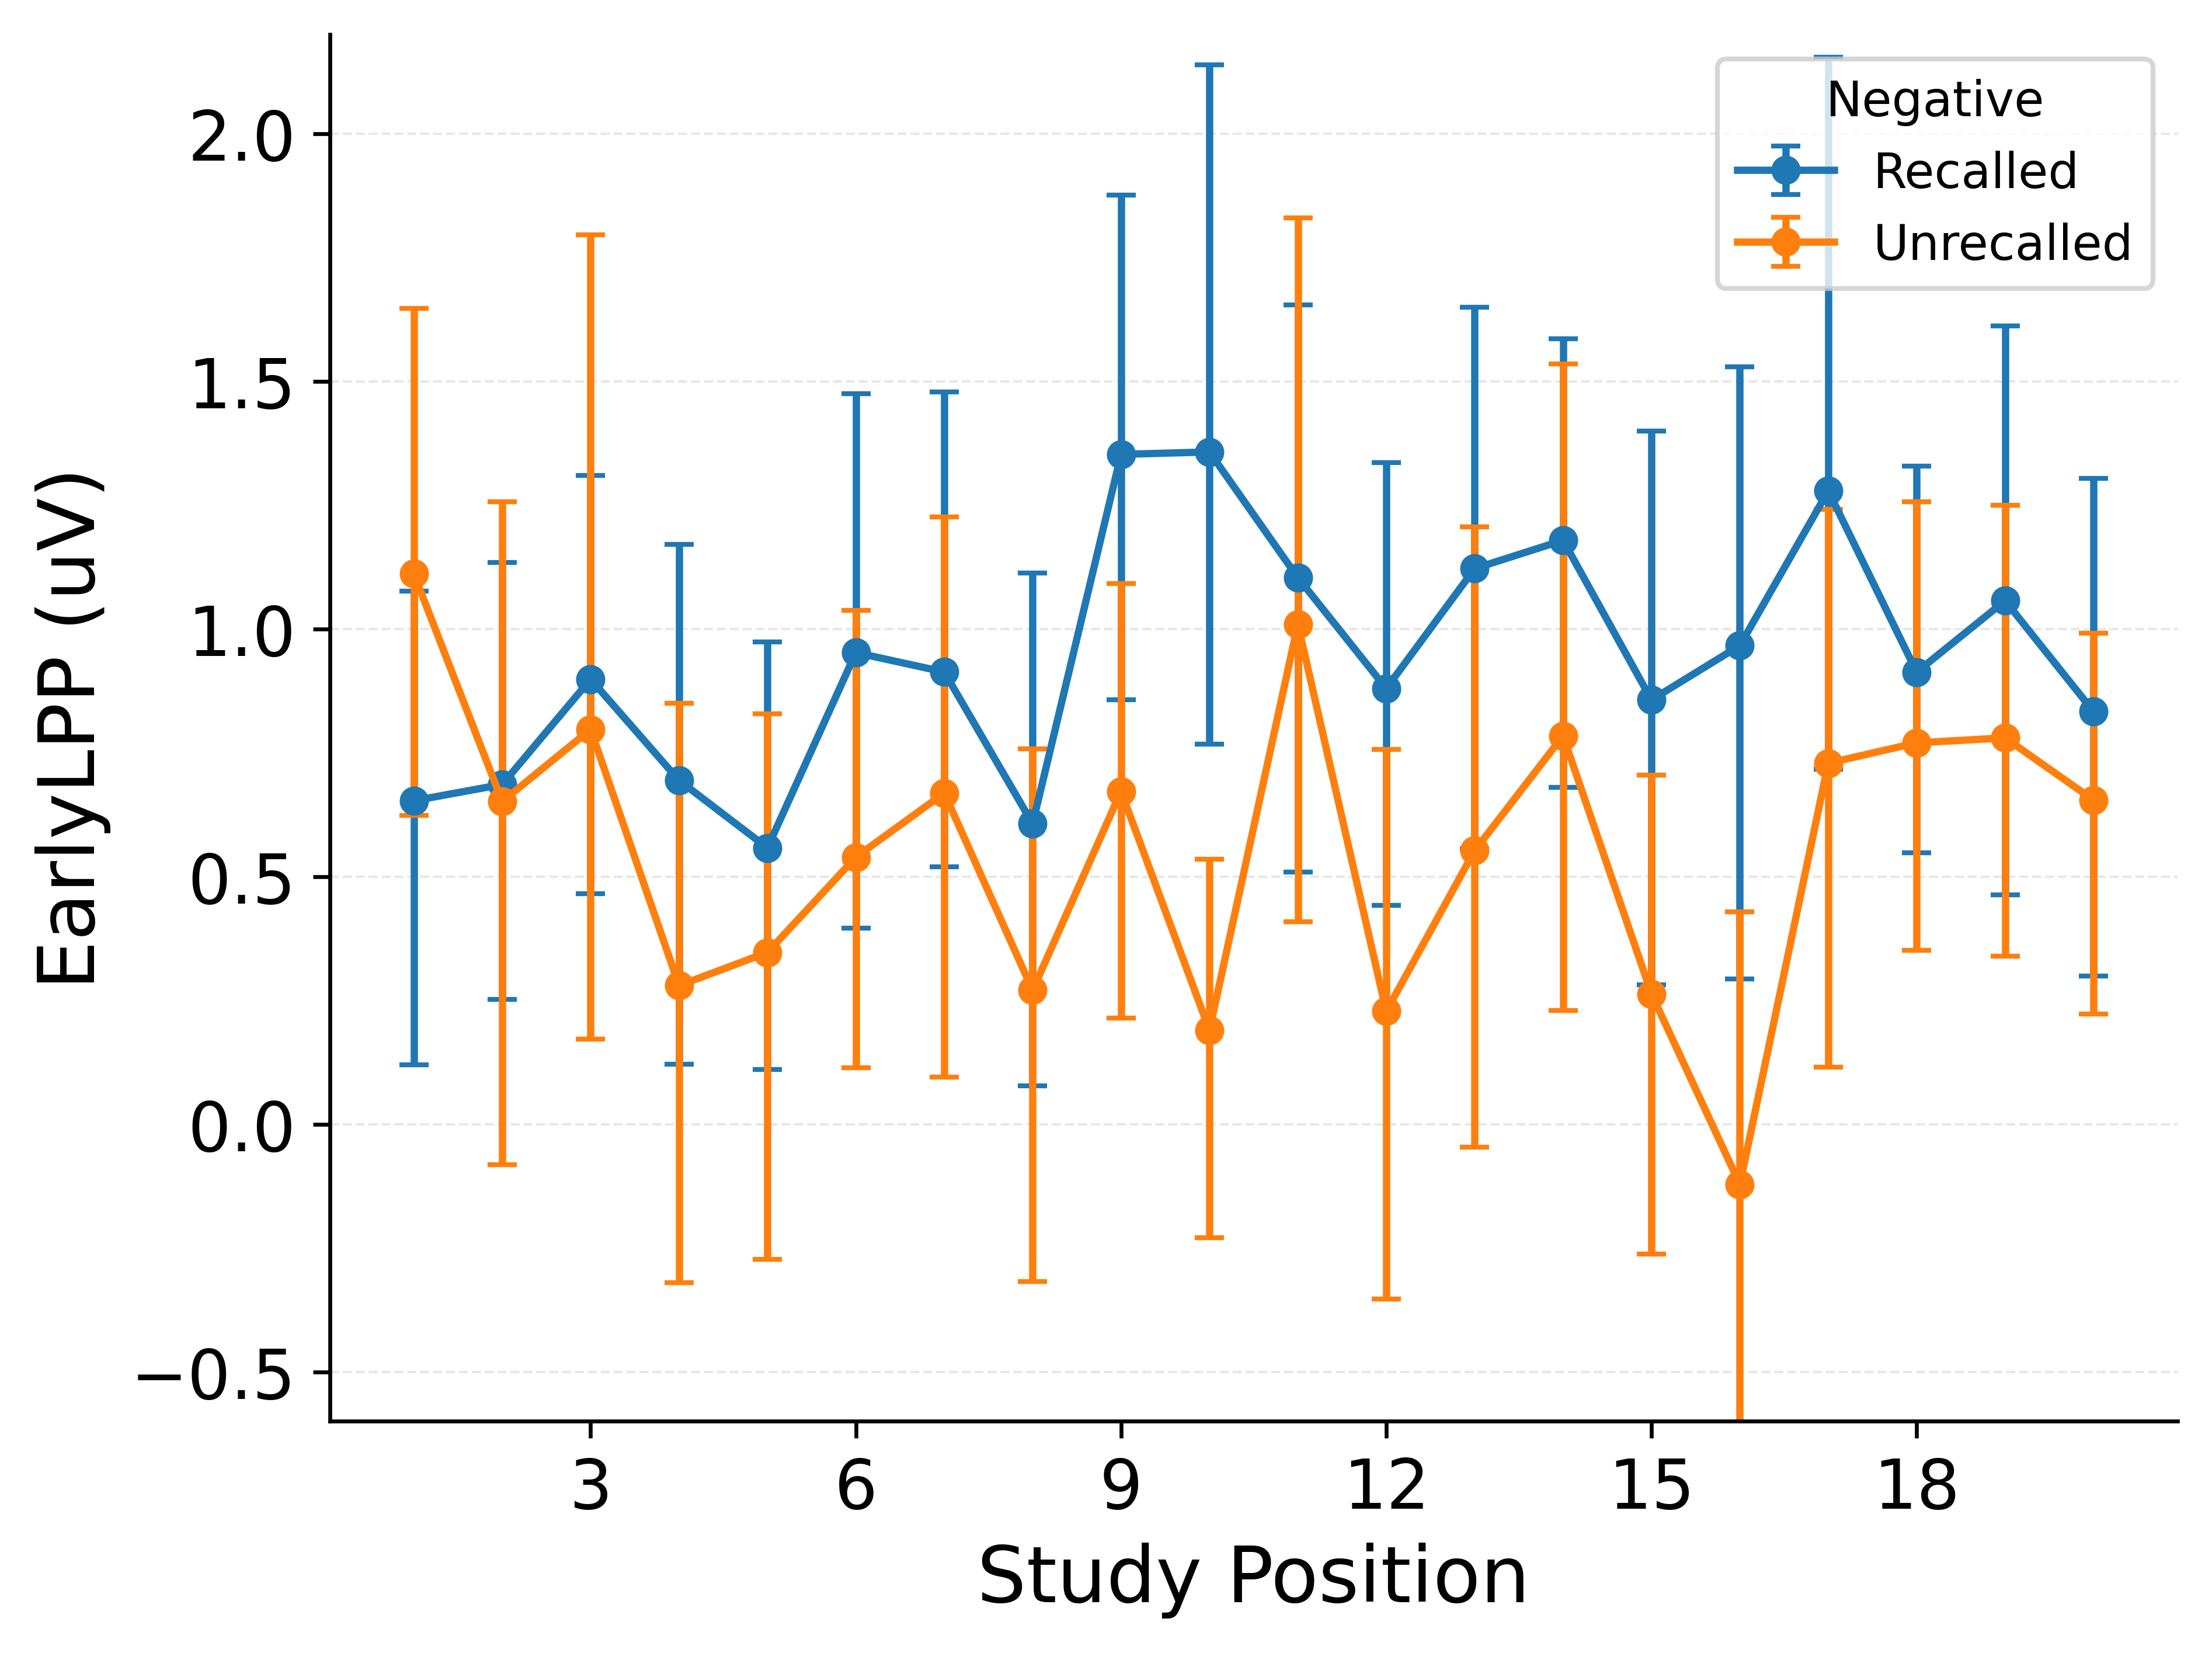
\includegraphics[keepaspectratio]{figures/analyses/cat_lpp_by_recall_EarlyLPP_Negative.png}}\end{minipage}%
%
\begin{minipage}{0.33\linewidth}
\pandocbounded{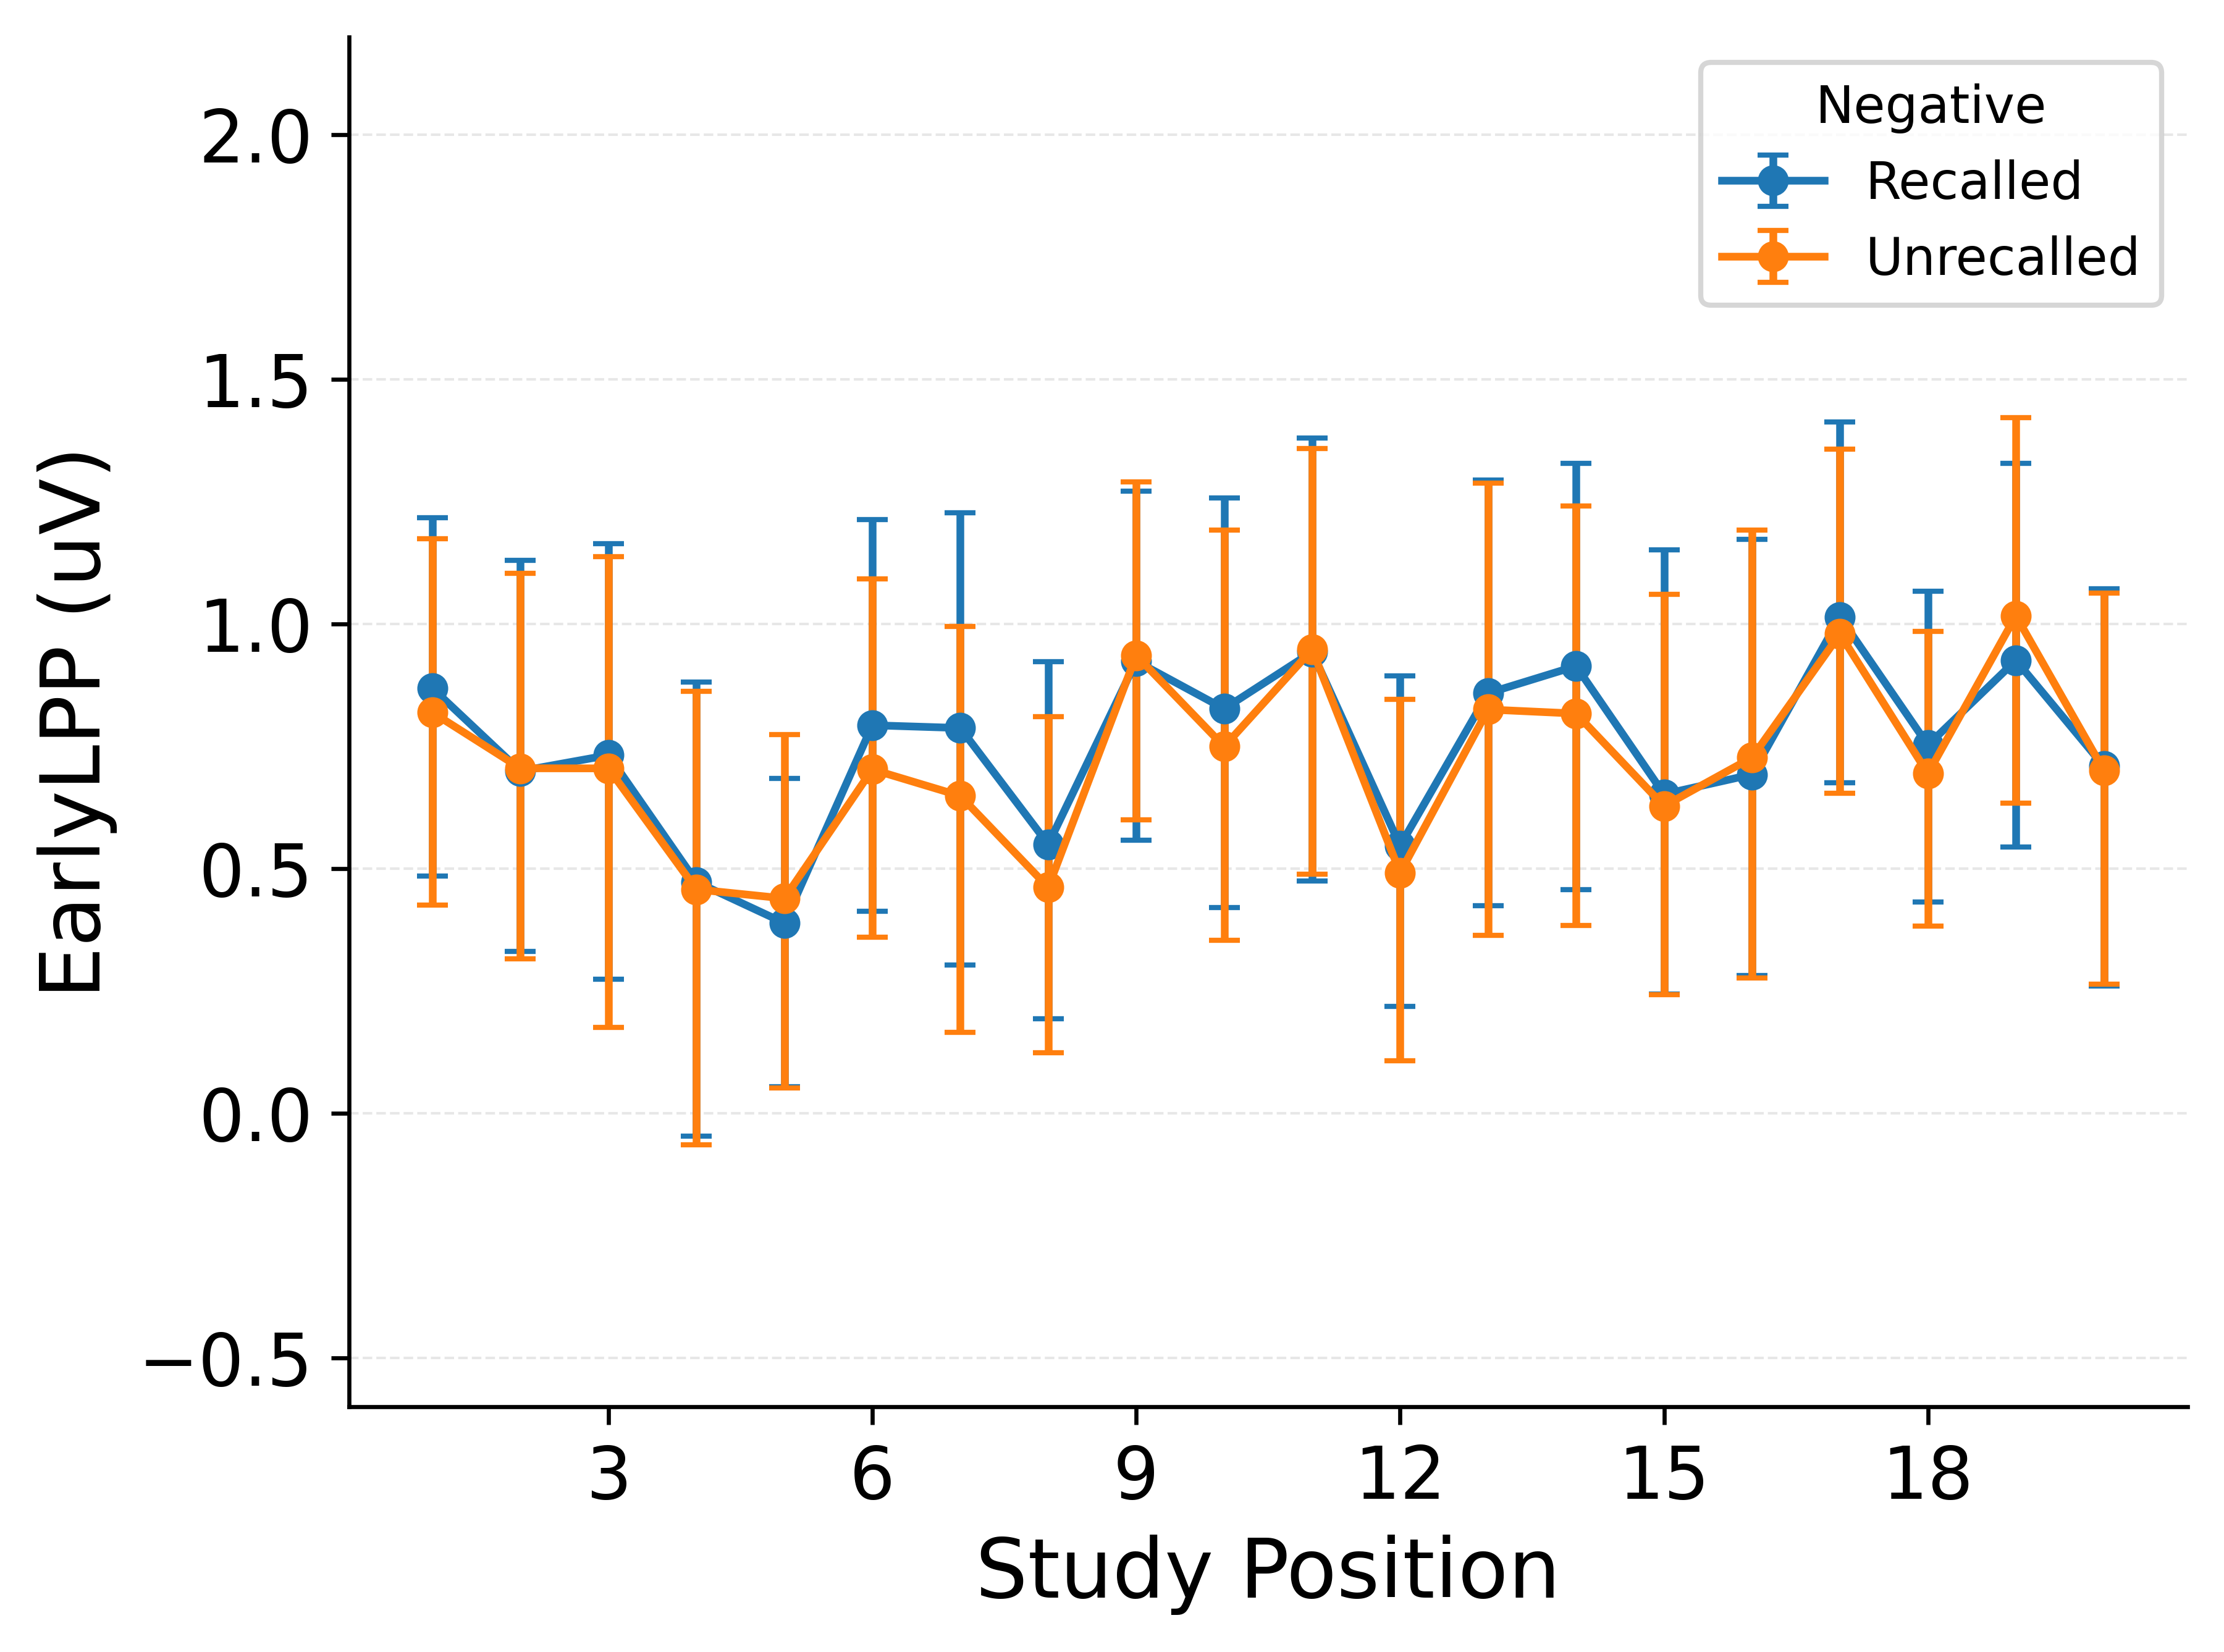
\includegraphics[keepaspectratio]{figures/fitting/TalmiEEG_WeirdCMRNoStop_50_set_likelihood_fixed_term_best_of_3_cat_lpp_by_recall_NEGATIVE_EARLYLPP.png}}\end{minipage}%
%
\begin{minipage}{0.33\linewidth}
\pandocbounded{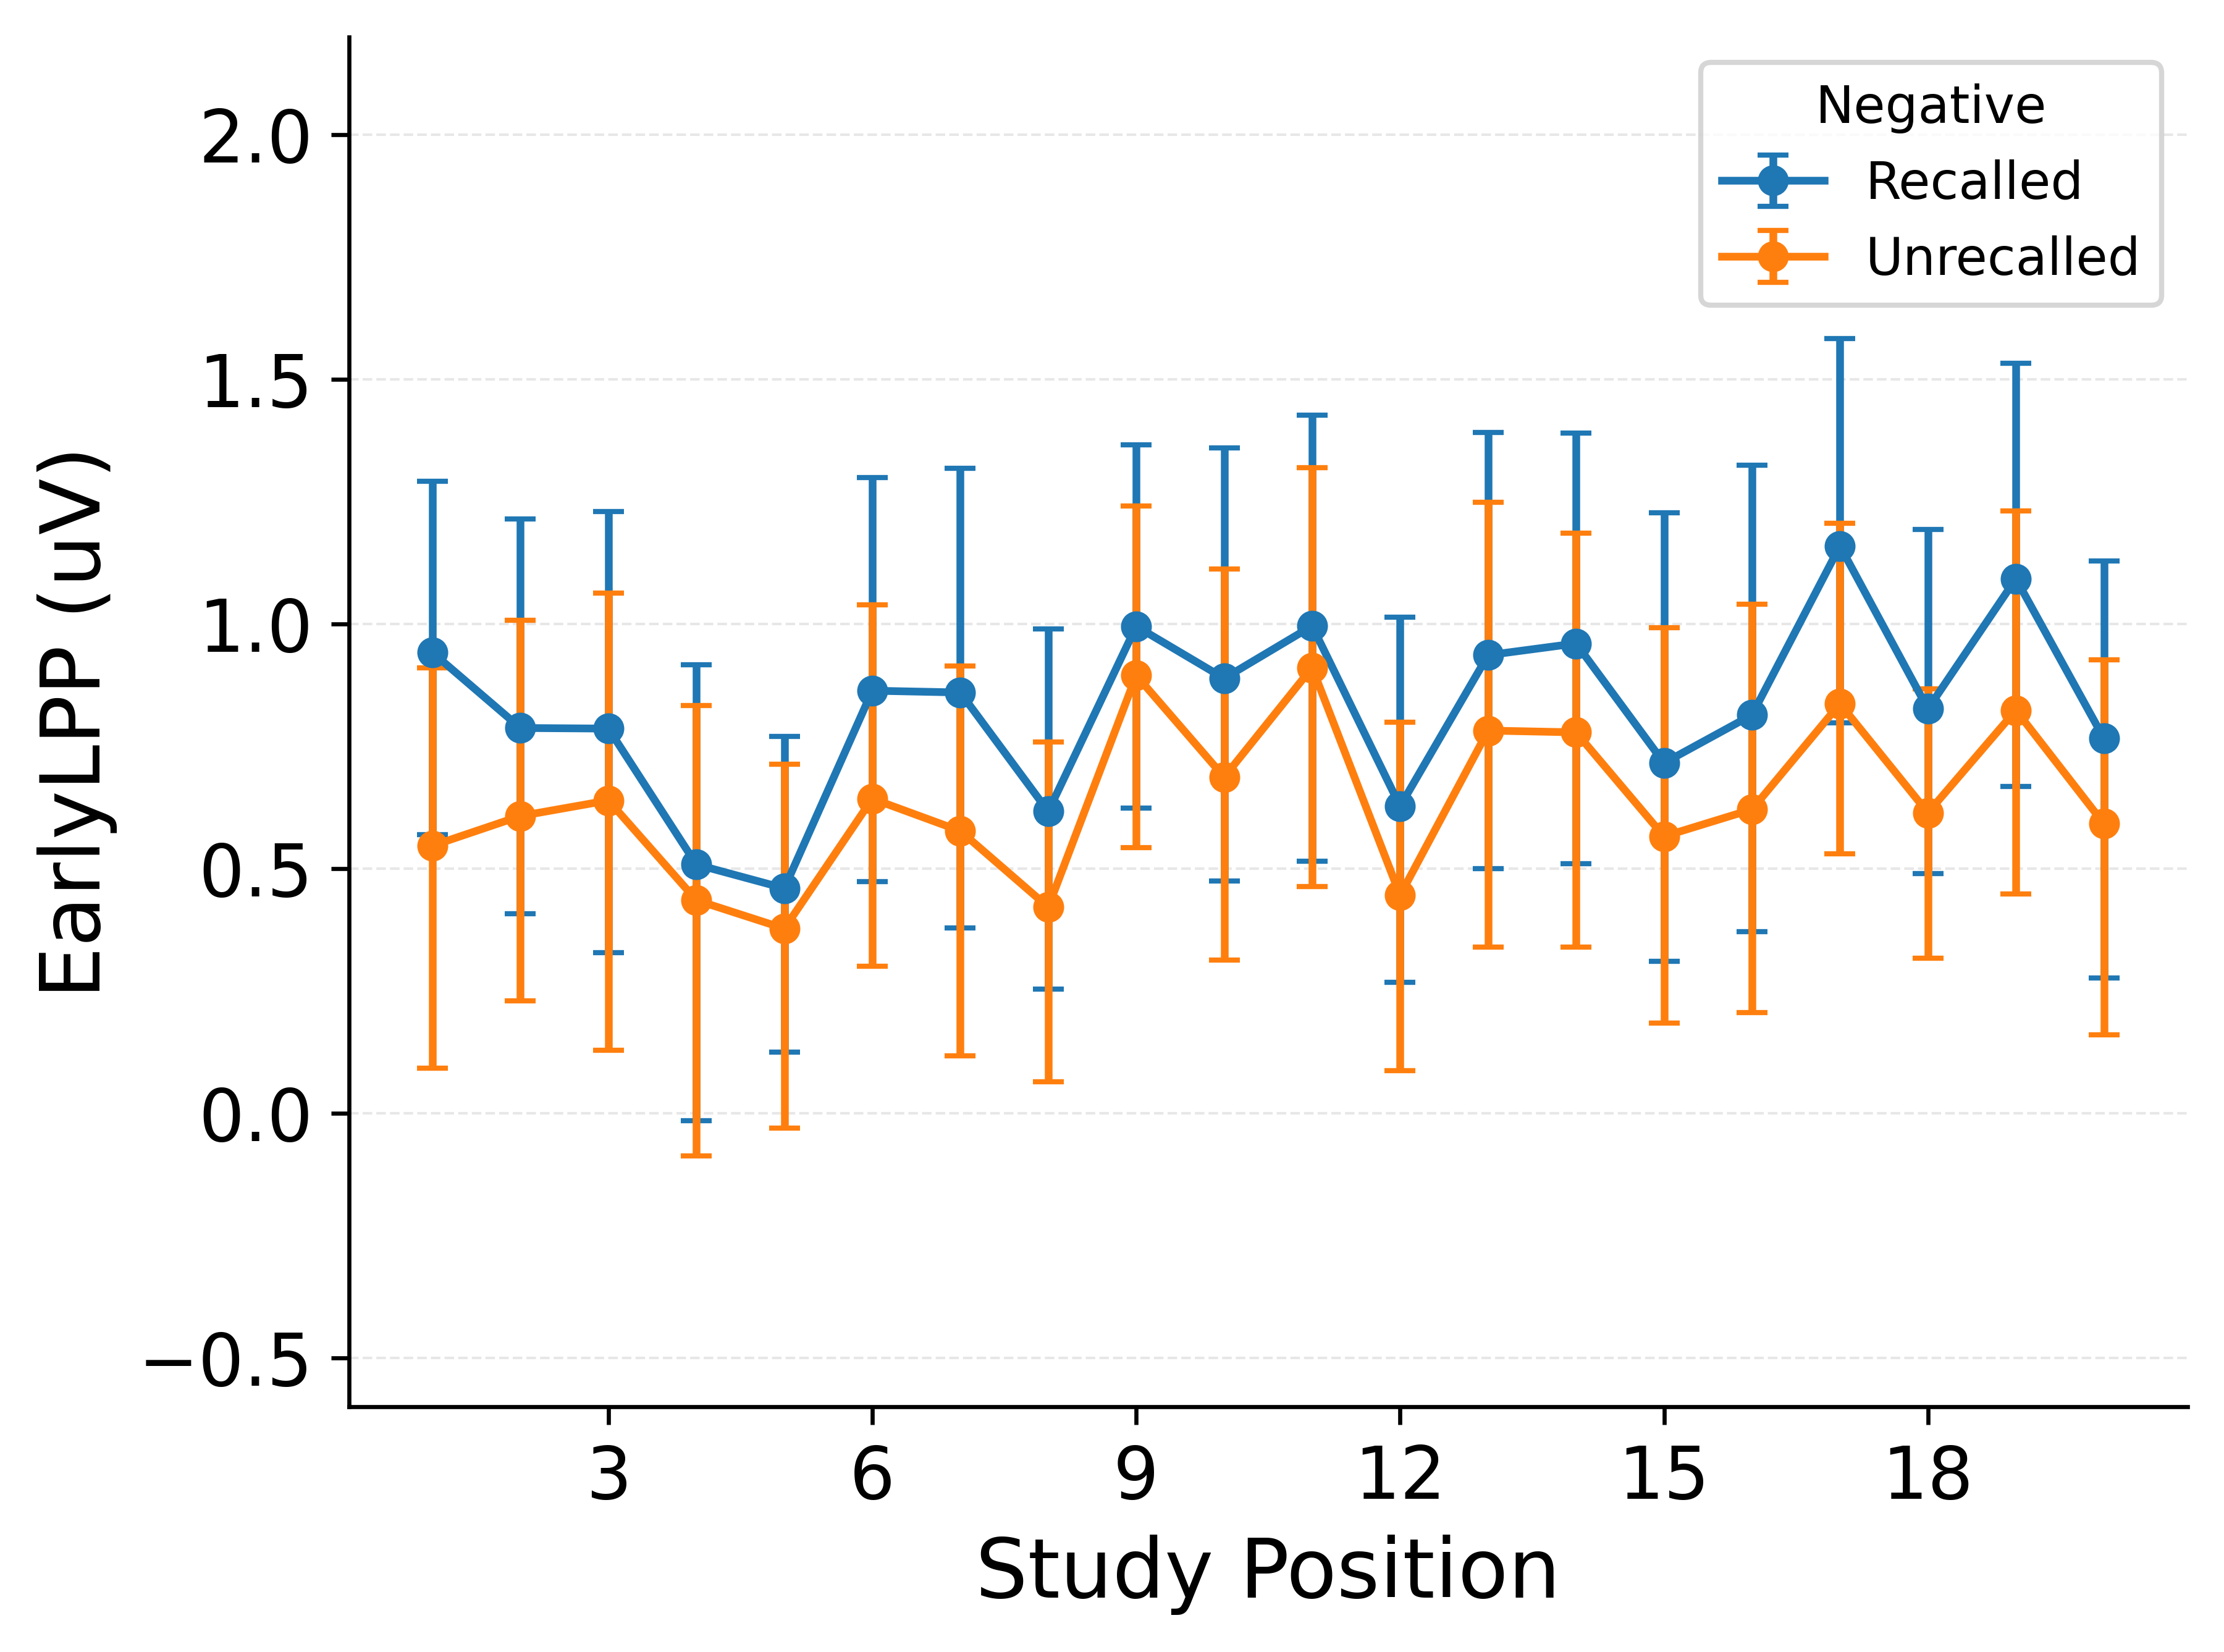
\includegraphics[keepaspectratio]{figures/fitting/TalmiEEG_EEGLPPParsimonious_50_set_likelihood_fixed_term_best_of_3_cat_lpp_by_recall_NEGATIVE_EARLYLPP.png}}\end{minipage}%
\newline
\begin{minipage}{0.33\linewidth}
\pandocbounded{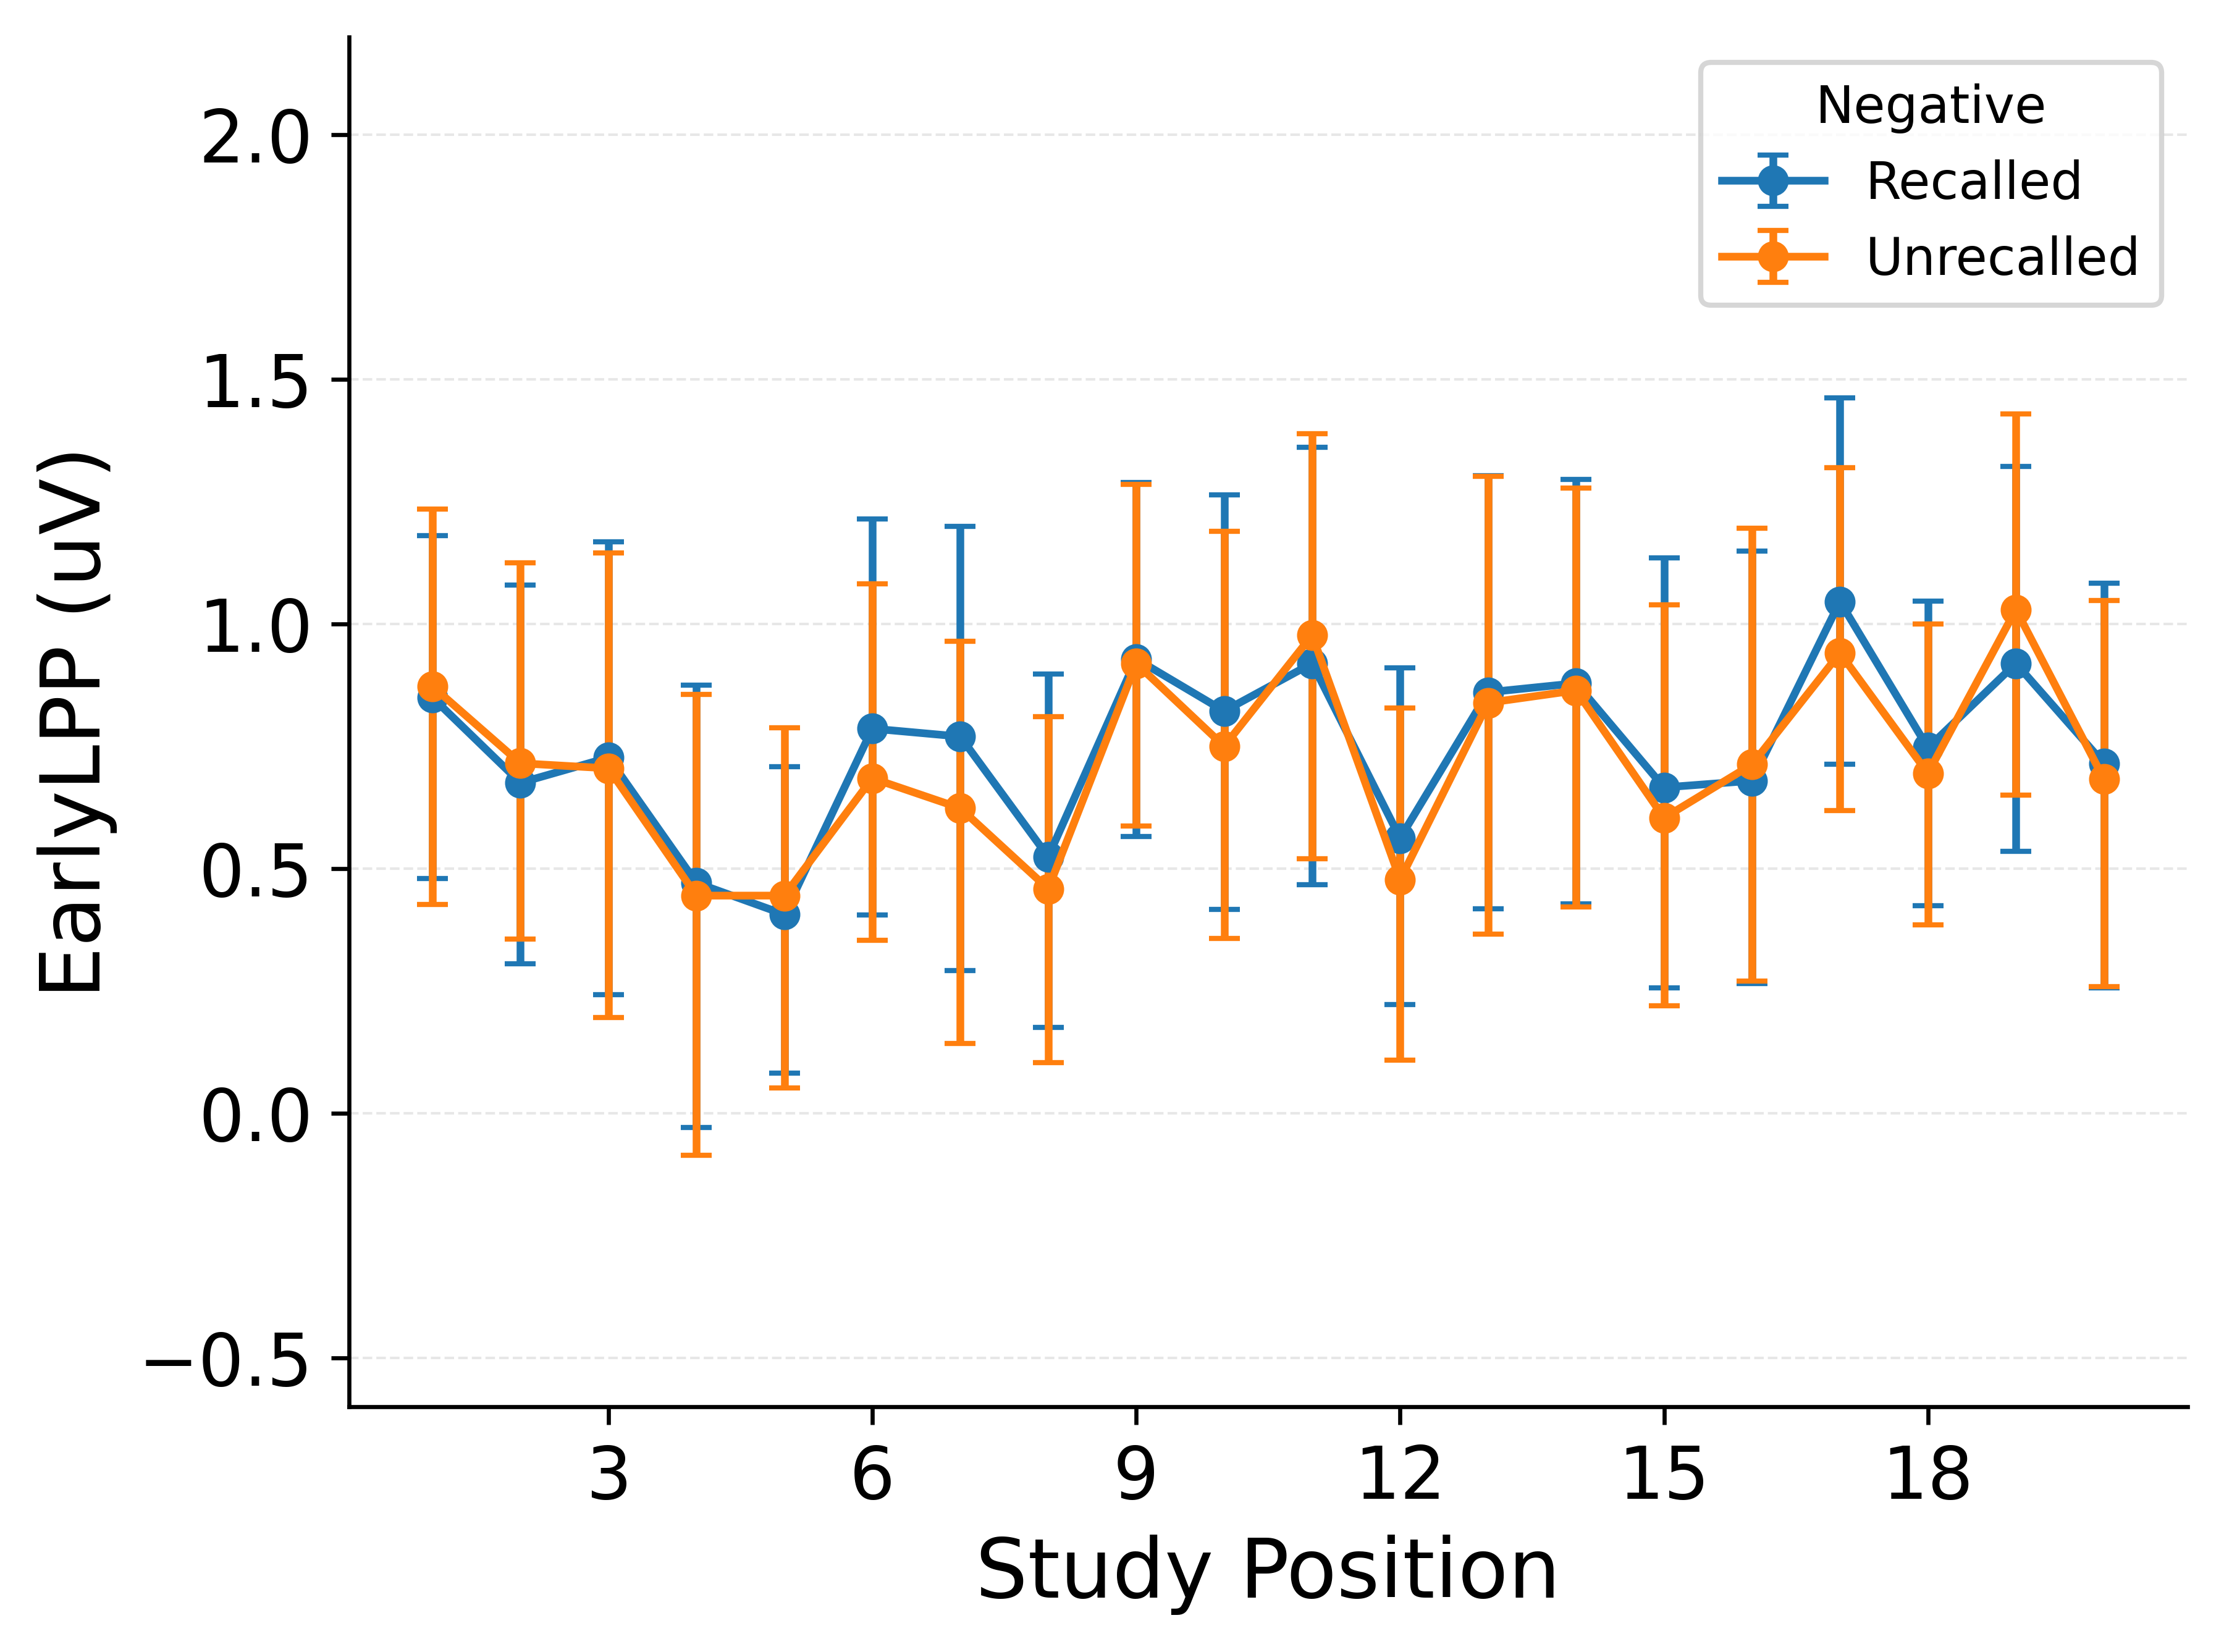
\includegraphics[keepaspectratio]{figures/fitting/TalmiEEG_eCMREmotionOnly_20260309_50_set_likelihood_best_of_3_cat_lpp_by_recall_NEGATIVE_EARLYLPP.png}}\end{minipage}%
%
\begin{minipage}{0.33\linewidth}
\pandocbounded{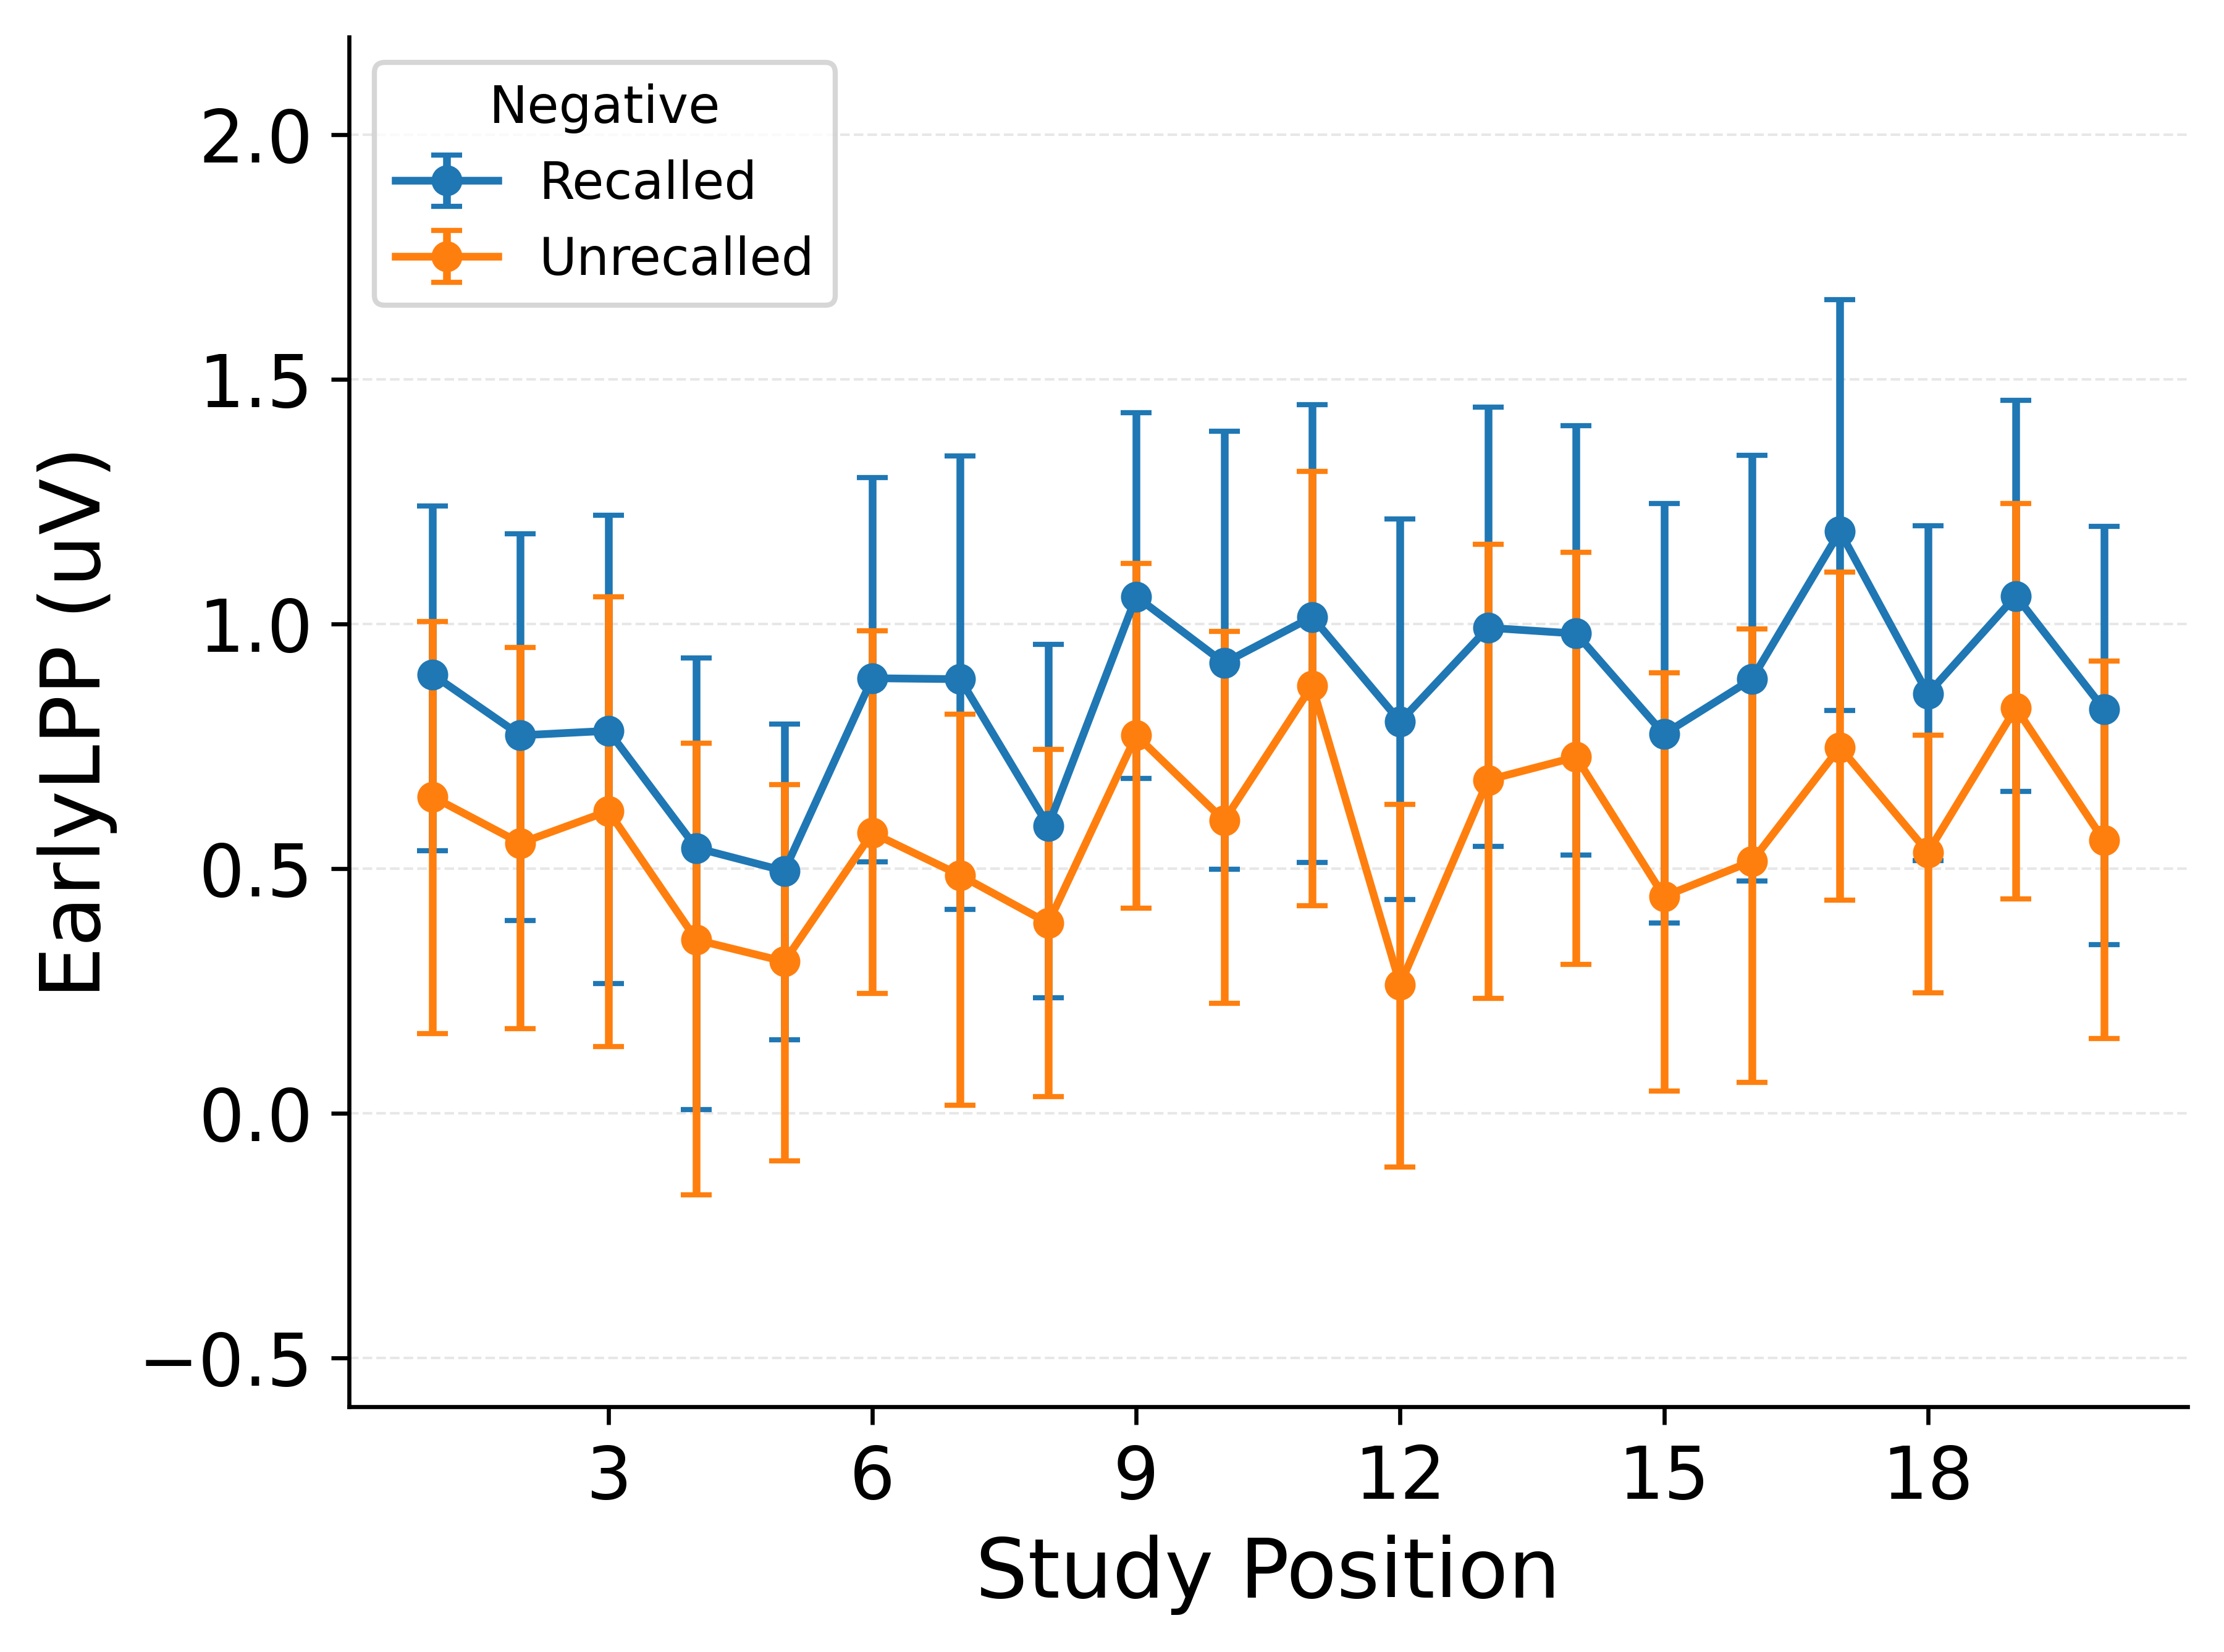
\includegraphics[keepaspectratio]{figures/fitting/TalmiEEG_eCMREmotionTimesLPP_20260309_50_set_likelihood_best_of_3_cat_lpp_by_recall_NEGATIVE_EARLYLPP.png}}\end{minipage}%

\end{figure}%

\subsection{Discussion}\label{discussion}

\subsection{References}\label{references}

\phantomsection\label{refs}
\begin{CSLReferences}{1}{0}
\bibitem[\citeproctext]{ref-anderson2005affective}
Anderson, A. K. (2005). Affective influences on the attentional dynamics
supporting awareness. \emph{Journal of Experimental Psychology:
General}, \emph{134}(2), 258--281.
\url{https://doi.org/10.1037/0096-3445.134.2.258}

\bibitem[\citeproctext]{ref-barnacle2018context}
Barnacle, G. E., Tsivilis, D., Schaefer, A., \& Talmi, D. (2018). Local
context influences memory for emotional stimuli but not
electrophysiological markers of emotion-dependent attention.
\emph{Psychophysiology}, \emph{55}(4), e13014.
\url{https://doi.org/10.1111/psyp.13014}

\bibitem[\citeproctext]{ref-bates2015lme4}
Bates, D., Mächler, M., Bolker, B., \& Walker, S. (2015). Fitting linear
mixed-effects models using lme4. \emph{Journal of Statistical Software},
\emph{67}(1), 1--48. \url{https://doi.org/10.18637/jss.v067.i01}

\bibitem[\citeproctext]{ref-chun2007interactions}
Chun, M. M., \& Turk-Browne, N. B. (2007). Interactions between
attention and memory. \emph{Current Opinion in Neurobiology},
\emph{17}(2), 177--184. \url{https://doi.org/10.1016/j.conb.2007.03.005}

\bibitem[\citeproctext]{ref-cuthbert2000brain}
Cuthbert, B. N., Schupp, H. T., Bradley, M. M., Birbaumer, N., \& Lang,
P. J. (2000). Brain potentials in affective picture processing:
Covariation with autonomic arousal and affective report.
\emph{Biological Psychology}, \emph{52}(2), 95--111.
\url{https://doi.org/10.1016/S0301-0511(99)00044-7}

\bibitem[\citeproctext]{ref-danglauser2011geneva}
Dan-Glauser, E. S., \& Scherer, K. R. (2011). The geneva affective
picture database ({GAPED}): A new 730-picture database focusing on
valence and normative significance. \emph{Behavior Research Methods},
\emph{43}(2), 468--477. \url{https://doi.org/10.3758/s13428-011-0064-1}

\bibitem[\citeproctext]{ref-delorme2004eeglab}
Delorme, A., \& Makeig, S. (2004). {EEGLAB}: An open source toolbox for
analysis of single-trial {EEG} dynamics including independent component
analysis. \emph{Journal of Neuroscience Methods}, \emph{134}(1), 9--21.
\url{https://doi.org/10.1016/j.jneumeth.2003.10.009}

\bibitem[\citeproctext]{ref-dolcos2002event}
Dolcos, F., \& Cabeza, R. (2002). Event-related potentials of emotional
memory: Encoding pleasant, unpleasant, and neutral pictures.
\emph{Cognitive, Affective, \& Behavioral Neuroscience}, \emph{2}(3),
252--263. \url{https://doi.org/10.3758/CABN.2.3.252}

\bibitem[\citeproctext]{ref-fields2023p300}
Fields, E. C. (2023). The {P300}, the {LPP}, context updating, and
memory: What is the functional significance of the emotion-related late
positive potential? \emph{International Journal of Psychophysiology},
\emph{192}, 43--52. \url{https://doi.org/10.1016/j.ijpsycho.2023.08.005}

\bibitem[\citeproctext]{ref-folkerts2018human}
Folkerts, S., Rutishauser, U., \& Howard, M. W. (2018). Human episodic
memory retrieval is accompanied by a neural contiguity effect. \emph{The
Journal of Neuroscience}, \emph{38}(17), 4200--4211.
\url{https://doi.org/10.1523/JNEUROSCI.2312-17.2018}

\bibitem[\citeproctext]{ref-fox2019companion}
Fox, J., \& Weisberg, S. (2019). \emph{An {R} companion to applied
regression} (3rd ed.). Sage Publications.

\bibitem[\citeproctext]{ref-hajcak2020significance}
Hajcak, G., \& Foti, D. (2020). Significance?... {Significance}!
{Empirical}, methodological, and theoretical connections between the
late positive potential and {P300} as neural responses to stimulus
significance: An integrative review. \emph{Psychophysiology},
\emph{57}(7), e13570. \url{https://doi.org/10.1111/psyp.13570}

\bibitem[\citeproctext]{ref-hajcak2010event}
Hajcak, G., MacNamara, A., \& Olvet, D. M. (2010). Event-related
potentials, emotion, and emotion regulation: An integrative review.
\emph{Developmental Neuropsychology}, \emph{35}(2), 129--155.
\url{https://doi.org/10.1080/87565640903526504}

\bibitem[\citeproctext]{ref-healey2016four}
Healey, M. K., \& Kahana, M. J. (2016). A four-component model of
age-related memory change. \emph{Psychological Review}, \emph{123}(1),
23--69. \url{https://doi.org/10.1037/rev0000015}

\bibitem[\citeproctext]{ref-healey2019contiguity}
Healey, M. K., Long, N. M., \& Kahana, M. J. (2019). Contiguity in
episodic memory. \emph{Psychonomic Bulletin \& Review}, \emph{26}(3),
699--720. \url{https://doi.org/10.3758/s13423-018-1537-3}

\bibitem[\citeproctext]{ref-howard2002distributed}
Howard, M. W., \& Kahana, M. J. (2002). A distributed representation of
temporal context. \emph{Journal of Mathematical Psychology},
\emph{46}(3), 269--299. \url{https://doi.org/10.1006/jmps.2001.1388}

\bibitem[\citeproctext]{ref-kragel2021distinct}
Kragel, J. E., Ezzyat, Y., Lega, B. C., Sperling, M. R., Worrell, G. A.,
Gross, R. E., Jobst, B. C., Sheth, S. A., Zaghloul, K. A., Stein, J. M.,
\& Kahana, M. J. (2021). Distinct cortical systems reinstate the content
and context of episodic memories. \emph{Nature Communications},
\emph{12}, 4444. \url{https://doi.org/10.1038/s41467-021-24393-1}

\bibitem[\citeproctext]{ref-lang2005international}
Lang, P. J., Bradley, M. M., \& Cuthbert, B. N. (2005).
\emph{International affective picture system ({IAPS}): Affective ratings
of pictures and instruction manual}. University of Florida.

\bibitem[\citeproctext]{ref-lenth2024emmeans}
Lenth, R. V. (2024). \emph{Emmeans: Estimated marginal means, aka
least-squares means}. \url{https://CRAN.R-project.org/package=emmeans}

\bibitem[\citeproctext]{ref-lohnas2021role}
Lohnas, L. J., \& Healey, M. K. (2021). The role of context in episodic
memory: Behavior and neurophysiology. In \emph{Psychology of learning
and motivation} (Vol. 75, pp. 157--199). Elsevier.
\url{https://doi.org/10.1016/bs.plm.2021.06.003}

\bibitem[\citeproctext]{ref-lohnas2015expanding}
Lohnas, L. J., Polyn, S. M., \& Kahana, M. J. (2015). Expanding the
scope of memory search: Modeling intralist and interlist effects in free
recall. \emph{Psychological Review}, \emph{122}(2), 337--363.
\url{https://doi.org/10.1037/a0039036}

\bibitem[\citeproctext]{ref-mackay2004emotion}
MacKay, D. G., Shafto, M., Taylor, J. K., Marian, D. E., Abrams, L., \&
Dyer, J. R. (2004). Relations between emotion, memory, and attention:
Evidence from taboo {Stroop}, lexical decision, and immediate memory
tasks. \emph{Memory \& Cognition}, \emph{32}(3), 474--488.
\url{https://doi.org/10.3758/BF03195840}

\bibitem[\citeproctext]{ref-macleod2017left}
MacLeod, C. A., \& Donaldson, D. I. (2017). Investigating the functional
utility of the left parietal {ERP} old/new effect: Brain activity
predicts within but not between participant variance in episodic
recollection. \emph{Frontiers in Human Neuroscience}, \emph{11}, 580.
\url{https://doi.org/10.3389/fnhum.2017.00580}

\bibitem[\citeproctext]{ref-manning2011oscillatory}
Manning, J. R., Polyn, S. M., Baltuch, G. H., Litt, B., \& Kahana, M. J.
(2011). Oscillatory patterns in temporal lobe reveal context
reinstatement during memory search. \emph{Proceedings of the National
Academy of Sciences}, \emph{108}(31), 12893--12897.
\url{https://doi.org/10.1073/pnas.1015174108}

\bibitem[\citeproctext]{ref-maris2007nonparametric}
Maris, E., \& Oostenveld, R. (2007). Nonparametric statistical testing
of {EEG}- and {MEG}-data. \emph{Journal of Neuroscience Methods},
\emph{164}(1), 177--190.
\url{https://doi.org/10.1016/j.jneumeth.2007.03.024}

\bibitem[\citeproctext]{ref-mather2011arousal}
Mather, M., \& Sutherland, M. R. (2011). Arousal-biased competition in
perception and memory. \emph{Perspectives on Psychological Science},
\emph{6}(2), 114--133. \url{https://doi.org/10.1177/1745691611400234}

\bibitem[\citeproctext]{ref-moran2013psychometric}
Moran, T. P., Jendrusina, A. A., \& Moser, J. S. (2013). The
psychometric properties of the late positive potential during emotion
processing and regulation. \emph{Brain Research}, \emph{1516}, 66--75.
\url{https://doi.org/10.1016/j.brainres.2013.04.018}

\bibitem[\citeproctext]{ref-nolan2010faster}
Nolan, H., Whelan, R., \& Reilly, R. B. (2010). {FASTER}: Fully
automated statistical thresholding for {EEG} artifact rejection.
\emph{Journal of Neuroscience Methods}, \emph{192}(1), 152--162.
\url{https://doi.org/10.1016/j.jneumeth.2010.07.015}

\bibitem[\citeproctext]{ref-olofsson2008affective}
Olofsson, J. K., Nordin, S., Sequeira, H., \& Polich, J. (2008).
Affective picture processing: An integrative review of {ERP} findings.
\emph{Biological Psychology}, \emph{77}(3), 247--265.
\url{https://doi.org/10.1016/j.biopsycho.2007.11.006}

\bibitem[\citeproctext]{ref-oostenveld2011fieldtrip}
Oostenveld, R., Fries, P., Maris, E., \& Schoffelen, J.-M. (2011).
{FieldTrip}: Open source software for advanced analysis of {MEG}, {EEG},
and invasive electrophysiological data. \emph{Computational Intelligence
and Neuroscience}, \emph{2011}, 156869.
\url{https://doi.org/10.1155/2011/156869}

\bibitem[\citeproctext]{ref-polyn2005category}
Polyn, S. M., Natu, V. S., Cohen, J. D., \& Norman, K. A. (2005).
Category-specific cortical activity precedes retrieval during memory
search. \emph{Science}, \emph{310}(5756), 1963--1966.
\url{https://doi.org/10.1126/science.1117645}

\bibitem[\citeproctext]{ref-polyn2009context}
Polyn, S. M., Norman, K. A., \& Kahana, M. J. (2009). A context
maintenance and retrieval model of organizational processes in free
recall. \emph{Psychological Review}, \emph{116}(1), 129--156.
\url{https://doi.org/10.1037/a0014420}

\bibitem[\citeproctext]{ref-pourtois2013brain}
Pourtois, G., Schettino, A., \& Vuilleumier, P. (2013). Brain mechanisms
for emotional influences on perception and attention: What is magic and
what is not. \emph{Biological Psychology}, \emph{92}(3), 492--512.
\url{https://doi.org/10.1016/j.biopsycho.2012.02.007}

\bibitem[\citeproctext]{ref-riberto2022neural}
Riberto, M., Paz, R., Pobric, G., \& Talmi, D. (2022). The neural
representations of emotional experiences are more similar than those of
neutral experiences. \emph{The Journal of Neuroscience}, \emph{42}(13),
2772--2785. \url{https://doi.org/10.1523/JNEUROSCI.1490-21.2022}

\bibitem[\citeproctext]{ref-rigoux2014bayesian}
Rigoux, L., Stephan, K. E., Friston, K. J., \& Daunizeau, J. (2014).
Bayesian model selection for group studies---revisited.
\emph{NeuroImage}, \emph{84}, 971--985.
\url{https://doi.org/10.1016/j.neuroimage.2013.08.065}

\bibitem[\citeproctext]{ref-rosenfeld2019p300}
Rosenfeld, J. P. (2020). P300 in detecting concealed information and
deception: A review. \emph{Psychophysiology}, \emph{57}(7), e13362.
\url{https://doi.org/10.1111/psyp.13362}

\bibitem[\citeproctext]{ref-sander2005systems}
Sander, D., Grandjean, D., \& Scherer, K. R. (2005). A systems approach
to appraisal mechanisms in emotion. \emph{Neural Networks},
\emph{18}(4), 317--352.
\url{https://doi.org/10.1016/j.neunet.2005.03.001}

\bibitem[\citeproctext]{ref-sassenhagen2019cluster}
Sassenhagen, J., \& Draschkow, D. (2019). Cluster-based permutation
tests of {MEG}/{EEG} data do not establish significance of effect
latency or location. \emph{Psychophysiology}, \emph{56}(6), e13335.
\url{https://doi.org/10.1111/psyp.13335}

\bibitem[\citeproctext]{ref-schindler2020selective}
Schindler, S., \& Straube, T. (2020). Selective visual attention to
emotional pictures: Interactions of task-relevance and emotion are
restricted to the late positive potential. \emph{Psychophysiology},
\emph{57}(9), e13585. \url{https://doi.org/10.1111/psyp.13585}

\bibitem[\citeproctext]{ref-schupp2000affective}
Schupp, H. T., Cuthbert, B. N., Bradley, M. M., Cacioppo, J. T., Ito,
T., \& Lang, P. J. (2000). Affective picture processing: The late
positive potential is modulated by motivational relevance.
\emph{Psychophysiology}, \emph{37}(2), 257--261.
\url{https://doi.org/10.1111/1469-8986.3720257}

\bibitem[\citeproctext]{ref-schupp2006emotion}
Schupp, H. T., Flaisch, T., Stockburger, J., \& Junghöfer, M. (2006).
Emotion and attention: Event-related brain potential studies. In
\emph{Progress in brain research} (Vol. 156, pp. 31--51).
\url{https://doi.org/10.1016/S0079-6123(06)56002-9}

\bibitem[\citeproctext]{ref-schupp2021case}
Schupp, H. T., \& Kirmse, U. M. (2021). Case-by-case: Emotional stimulus
significance and the modulation of the {EPN} and {LPP}.
\emph{Psychophysiology}, \emph{58}(4), e13766.
\url{https://doi.org/10.1111/psyp.13766}

\bibitem[\citeproctext]{ref-sederberg2008context}
Sederberg, P. B., Howard, M. W., \& Kahana, M. J. (2008). A
context-based theory of recency and contiguity in free recall.
\emph{Psychological Review}, \emph{115}(4), 893--912.
\url{https://doi.org/10.1037/a0013396}

\bibitem[\citeproctext]{ref-stephan2009bayesian}
Stephan, K. E., Penny, W. D., Daunizeau, J., Moran, R. J., \& Friston,
K. J. (2009). Bayesian model selection for group studies.
\emph{NeuroImage}, \emph{46}(4), 1004--1017.
\url{https://doi.org/10.1016/j.neuroimage.2009.03.025}

\bibitem[\citeproctext]{ref-stephens2010autonomic}
Stephens, C. L., Christie, I. C., \& Friedman, B. H. (2010). Autonomic
specificity of basic emotions: Evidence from pattern classification and
cluster analysis. \emph{Biological Psychology}, \emph{84}(3), 463--473.
\url{https://doi.org/10.1016/j.biopsycho.2010.03.014}

\bibitem[\citeproctext]{ref-storn1997differential}
Storn, R., \& Price, K. (1997). Differential evolution -- a simple and
efficient heuristic for global optimization over continuous spaces.
\emph{Journal of Global Optimization}, \emph{11}(4), 341--359.
\url{https://doi.org/10.1023/A:1008202821328}

\bibitem[\citeproctext]{ref-talmi2013enhanced}
Talmi, D. (2013). Enhanced emotional memory: Cognitive and neural
mechanisms. \emph{Current Directions in Psychological Science},
\emph{22}(6), 430--436. \url{https://doi.org/10.1177/0963721413498893}

\bibitem[\citeproctext]{ref-talmi2019retrieved}
Talmi, D., Lohnas, L. J., \& Daw, N. D. (2019). A retrieved context
model of the emotional modulation of memory. \emph{Psychological
Review}, \emph{126}(4), 455--485.
\url{https://doi.org/10.1037/rev0000132}

\bibitem[\citeproctext]{ref-talmi2007contribution}
Talmi, D., Luk, B. T. C., McGarry, L. M., \& Moscovitch, M. (2007). The
contribution of relatedness and distinctiveness to emotionally-enhanced
memory. \emph{Journal of Memory and Language}, \emph{56}(4), 555--574.
\url{https://doi.org/10.1016/j.jml.2007.01.002}

\bibitem[\citeproctext]{ref-talmi2012accounting}
Talmi, D., \& McGarry, L. M. (2012). Accounting for immediate emotional
memory enhancement. \emph{Journal of Memory and Language}, \emph{66}(1),
93--108. \url{https://doi.org/10.1016/j.jml.2011.07.009}

\bibitem[\citeproctext]{ref-turner2016more}
Turner, B. M., Rodriguez, C. A., Norcia, T. M., McClure, S. M., \&
Steyvers, M. (2016). Why more is better: Simultaneous modeling of {EEG},
{fMRI}, and behavioral data. \emph{NeuroImage}, \emph{128}, 96--115.
\url{https://doi.org/10.1016/j.neuroimage.2015.12.030}

\bibitem[\citeproctext]{ref-weinberg2021emotion}
Weinberg, A., Correa, K. A., Stevens, E. S., \& Shankman, S. A. (2021).
The emotion-elicited late positive potential is stable across five
testing sessions. \emph{Psychophysiology}, \emph{58}(11), e13904.
\url{https://doi.org/10.1111/psyp.13904}

\bibitem[\citeproctext]{ref-wessa2010emopics}
Wessa, M., Kanske, P., Neumeister, P., Bode, K., Heissler, J., \&
Schönfelder, S. (2010). {EmoPics}: Subjektive und psychophysiologische
evaluationen neuen bildmaterials f{ü}r die klinisch-bio-psychologische
forschung. \emph{Zeitschrift f{ü}r Klinische Psychologie Und
Psychotherapie}, \emph{Supplement}(1/11), 77.

\bibitem[\citeproctext]{ref-zarubin2020contributions}
Zarubin, V. C., Phillips, T. K., Robertson, E., Bolton Swafford, P. G.,
Bunge, T., Aguillard, D., Martsberger, C., \& Mickley Steinmetz, K. R.
(2020). Contributions of arousal, attention, distinctiveness, and
semantic relatedness to enhanced emotional memory: An event-related
potential and electrocardiogram study. \emph{Affective Science},
\emph{1}(3), 172--185. \url{https://doi.org/10.1007/s42761-020-00012-y}

\end{CSLReferences}






\end{document}
